
\newcommand{\green}[1]{{\color{green} #1}}
\newcommand{\red}[1]{{\color{red} #1}}
\newcommand{\blue}[1]{{\color{blue} #1}}
\newcommand{\bendability}{\nu}

\newcommand{\upd}{\mathrm{d}}
\newcommand{\ddp}[2]{\frac{\partial #1}{\partial #2}}
\newcommand{\dd}[2]{\frac{\upd #1}{\upd #2}}
\newcommand{\xleft}{x_{-}}
\newcommand{\xright}{x_{+}}

%nb: you need \text{(\theequation)} rather than just (\theequation) if you want the equation number to be in same font as the text (e.g. sans serif)
\newcommand\abcdeqn[2]{\refstepcounter{equation}
     \[
     \label{#1}
     #2
     \eqno{\text{(\theequation)}\text{a,b,c,d}}
     \]
}
\newcommand\abeqn[2]{\refstepcounter{equation}
     \[
     \label{#1}
     #2
     \eqno{\text{(\theequation)}\text{a,b}}
     \]
}


\graphicspath{{./Sections/Chapter2_modelling/figures/}}


%%%%%%%%%%%%%%%%%%%%%%%%
\chapter{Modelling bendotaxis}
In this chapter, we develop and analyse a mathematical model of bendotaxis, motivated by the proof of concept experiments shown in \S1.4.3. We begin by deriving a two-dimensional theoretical model that combines linear elasticity to describe the channel deformations with lubrication theory to describe fluid flow in response to capillary-induced pressure gradient. We then describe a numerical scheme used to solve the model equations and discuss the behaviour of these solutions. Following this, we consider the case of small deflections -- in which analytical progress can be made -- and discuss the implications of our model for droplet removal from deformable channels by bendotaxis.

\section{Theoretical model of bendotaxis}
\begin{figure}[t]
\centering
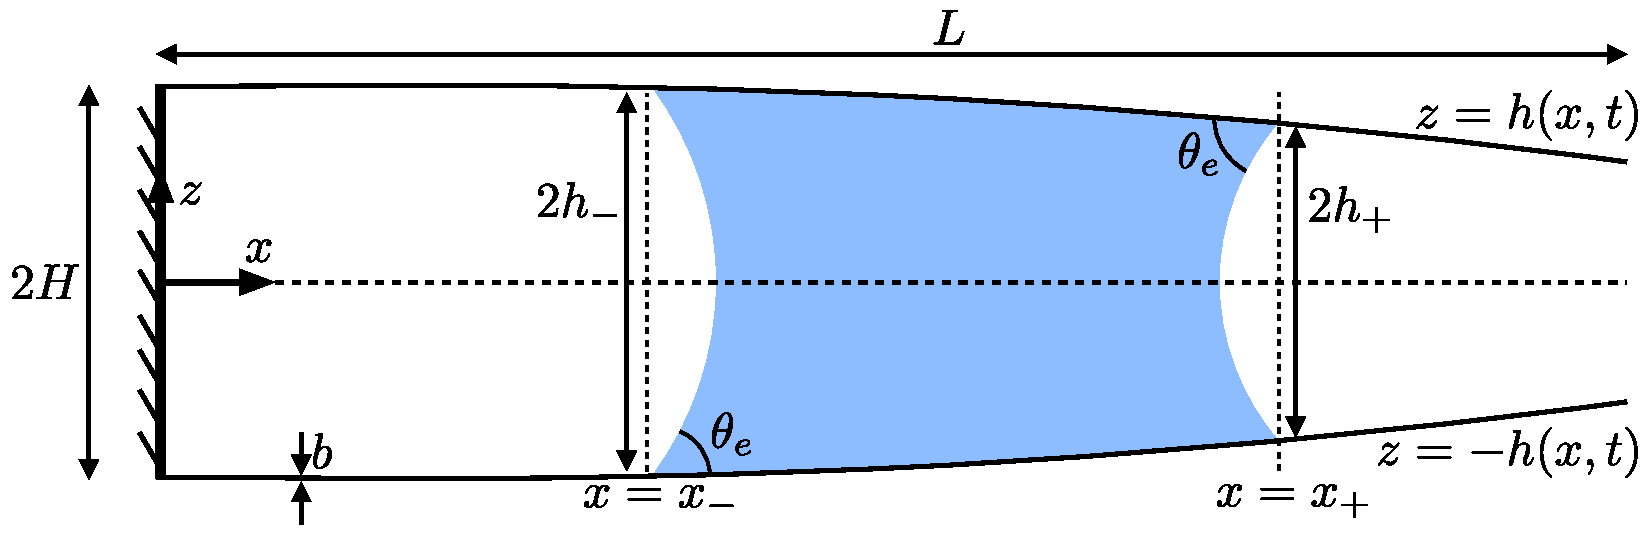
\includegraphics[width = 0.75\textwidth]{Schematic}
\label{fig:Model:Schematic}
\caption{Schematic of a droplet in a flexible channel which has underformed wall separation $2H$ and length $L$, and whose walls have thickness $b$. The menisci contact the walls at perpendicular distances $x = x_{-}(t)$ and $x = x_{+}(t)$ from the clamped end of the channel.}
\end{figure}

In this section, we develop a theoretical model of bendotaxis. We consider the setup shown in Figure~\ref{fig:Model:Schematic}; a channel bounded by two narrow, flexible beams of thickness $b$, length $L$, density $\rho_s$ and Young's modulus $E$, are clamped parallel to one another at a distance $2H$ apart, at one end of the beams. This clamped end defines the $z$-axis, and the axis of the channel (parallel to the undeformed beams) defines the $x$ axis. Although we shall show its effect to be negligible, gravity is initially assumed to act parallel to the $z$-axis.

The channel contains a droplet of liquid of viscosity $\mu$, surface tension $\gamma$ and density $\rho$. The droplet has (two dimensional) volume $\Omega$, and makes a liquid bridge between the channel walls, wetting them over of a region $\xleft(t) < x <\xright(t)$. We assume that the droplet makes a constant contact angle $\theta_e$ with the channel walls (i.e.~we neglect dynamic contact angle effects, and assume there is no contact angle hysteresis).

Table~\ref{T:Chapter2:ExptValues} contains typical experimental values from the experiments shown in Chapter 1 (and discussed further in Chapter 3) of those quantities introduced here.

\def\arraystretch{1.1}%stretch the table
\begin{table}[t]
\begin{center}
\begin{tabular}{| c | c | c | c  |}
\hline
Description & Symbol & Value & SI Units \\ \hline \hline
Droplet surface tension & $\gamma$ & $22\times 10^{-3}$ & N~m\textsuperscript{-1}\\
Young's modulus & $E$ & $63\times 10^9$ & Pa\\
Channel wall thickness & $b$ & $180\times 10^{-6}$ & m\\
Channel half width & $H$ &$ 250\times 10^{-6}$ & m\\
Channel length & $L$  & $25\times 10^{-3}$ &m\\
Liquid density & $\rho_l$ & $960$ & kg~m\textsuperscript{-3}\\
Channel wall density & $\rho_s$ & $2500$ & kg~m\textsuperscript{-3}\\
Droplet viscosity (dynamic) & $\mu$ & $0.096$ & Pa~s  \\
Droplet volume & $\Omega$ & $15\times 10^{-9}$ & m\textsuperscript{3} \\
Contact angle & $\theta_e$ & $0$ & n/a\\
Capillary time scale & $\tau_c$ & $10$ & s \\
Bendotaxis time scale & $\tau$ & $10$ & s\\ \hline
\end{tabular}
\end{center}
\caption{Summary of notation used in this chapter and typical values of the corresponding variables in the proof of concept experiment (\S1.4.3) and experimental study (Chapter 3). }\label{T:Chapter2:ExptValues}
\end{table}
\subsection{A scaling argument}\label{S:Model:Scaling}
Before we derive a detailed mathematical model, we consider a scaling argument, valid for small droplets, to gain theoretical insight.

As discussed in Chapter 1, we expect that droplet motion will be driven by the pressure gradient across it. This pressure gradient arises from a difference in Laplace pressure at the leading and rear menisci. When surface tension forces dominate over gravitational forces (i.e.~when the droplet Bond number is small), the menisci do not deform significantly under the weight of the liquid and they take the shape of semi-circular arcs with interfacial curvatures $\kappa_{\pm} = -\cos \theta_e/h_{\pm}$~\citep{deGennes2004}, where $h_{\pm}$ are the channel half widths at the menisci (Figure~\ref{fig:Model:Schematic}).

The corresponding liquid pressure at each meniscus is $p_{\pm} = -\gamma  \cos \theta_e/h_{\pm}$, and the pressure change across the droplet is
\begin{equation}\label{E:Chapter2:Model:Scaling:PressureChange}
\Delta P = p_{+} - p_{-} = -\gamma \cos \theta_e(1/h_{+} - 1/h_{-}).
\end{equation}

In the case that the droplet volume is small relative to the channel volume, $V = \Omega / (2HL) \ll 1$, the liquid pressure is applied to the beams over a relatively short length, and the resulting channel deformation will be small. The length $\Delta X = \xright - \xleft$ over which the pressure is applied is approximately $\Delta X \approx \Omega/(2H)$ -- equal to the length of the droplet in the undeformed channel -- and we can expand the channel width as
\begin{equation}\label{E:Chapter2:Model:Scaling:ChannelWidthDiff}
h_+ \sim h_- + \alpha \Delta X.
\end{equation}
Here $\alpha$ is the average channel slope across the droplet (whose scaling is to be determined).

Combining~\eqref{E:Chapter2:Model:Scaling:PressureChange} and~\eqref{E:Chapter2:Model:Scaling:ChannelWidthDiff}, the pressure gradient across the droplet can be approximated by
\begin{equation}\label{E:Chapter2:Model:Scaling:PressureChangeExpanded}
\frac{\Delta P}{\xright -  \xleft} \sim  \frac{\Delta P}{\Delta X} \sim \frac{ \alpha \gamma \cos \theta_e \Delta X }{H^2}.
\end{equation}

The channel walls are slender, so their resistance to bending is characterized by their bending stiffness $B = Eb^3/12$~\citep{Howell2009}, and their behaviour can be modelled using linear beam theory. Since the droplet is small, its effect on the channel can be approximated by a point force of magnitude $\gamma \cos \theta_e\Delta X /H$; linear beam theory~\citep{Howell2009} gives the scaling for the angle of a cantilever beam forced by a point force of this magnitude, and bending over a length scale $L$, as
\begin{equation}\label{E:Chapter2:Model:Scaling:AngleScaling}
\alpha \sim\frac{\gamma \cos \theta_e \Delta X}{H} \frac{L^2}{B}.
\end{equation}

Provided that the droplet aspect ratio $\Delta X /H$ is small, lubrication theory~\citep{Leal2007} is applicable for the fluid flow and gives the velocity scale $U$ for the fluid flow as
\begin{equation}\label{E:Chapter2:Model:Scaling:VelocityScale}
U \sim \frac{H^2}{\mu}\frac{\Delta P}{\Delta X}.
\end{equation}

Combining~\eqref{E:Chapter2:Model:Scaling:PressureChangeExpanded},~\eqref{E:Chapter2:Model:Scaling:AngleScaling} and~\eqref{E:Chapter2:Model:Scaling:VelocityScale} gives the time scale $\tau$ for a droplet to move along the length of the channel as
\begin{equation}\label{E:Chapter2:Model:Scaling:TimeScaling}
\tau \sim \frac{L}{U} \sim   \frac{\mu H B}{L \gamma^2 \cos^2 \theta_e \Delta X}.
\end{equation}

The other relevant time scale is the capillary time scale,
\begin{equation}\label{E:Chapter2:Model:Scaling:CapillaryTimeScale}
\tau_c = \frac{\mu L^2}{|\gamma\cos \theta_e| H},
\end{equation}
which can be thought of as the typical time taken for liquid of viscosity $\mu$ and surface tension $\gamma$ to imbibe a distance $L$ in a capillary tube of radius $H$~\citep{Washburn1921PhysRev}.

The ratio between these two time scales (\eqref{E:Chapter2:Model:Scaling:TimeScaling} and~\eqref{E:Chapter2:Model:Scaling:CapillaryTimeScale}) is
\begin{equation}\label{E:Chapter2:Model:Scaling:ScalingResult}
\frac{\tau}{\tau_c}\sim \frac{B}{|\gamma \cos \theta_e|\Delta X}\frac{H^2}{L^3}.
\end{equation}
Note that for relatively undeformable channels (large $B$ or small $\gamma$), this time scale becomes large, and decreases with increasing droplet size $\Delta X$. Perhaps surprisingly, however, $\tau$ decreases with increasing $H$ -- narrower channels exhibit faster bendotaxis. This is the reverse of imbibition, where the decrease in channel permeability with channel width $H$ is more than offset by the increase in capillary driving pressure -- the imbibition time~\eqref{E:Chapter2:Model:Scaling:CapillaryTimeScale} increases with decreasing $H$.

We now turn to our more detailed mathematical model, but we shall return to this scaling argument to understand the results of this model.
\subsection{Mathematical model}\label{S:Theoretical:Model}
We now derive a detailed mathematical model, beginning here with modelling of the flow within the channel. Note that, under the assumption that the channel is symmetric, we only need to consider its half-width, $h(x,t)$, as in Figure~\ref{fig:Model:Schematic}.

\subsubsection{Fluid motion}
We assume that the drop is long and thin, $\Delta X/H \ll 1$, so that lubrication theory~\citep{Leal2007} applies. Within this framework, the local conservation of mass combined with the kinematic boundary condition at the channel walls ensures that the droplet pressure $p(x,t)$ satisfies
\begin{equation}\label{E:Chapter2:Model:MathModel:Fluid:Reynolds}
\ddp{h}{t} = \frac{1}{3\mu}\ddp{}{x}\left(h^3\ddp{p}{x}\right) \qquad \xleft(t) < x < \xright(t).
\end{equation}

We assume that evaporation is negligible. The time scale of evaporation for a sessile droplet on a substrate is $\tau_{e} \sim \rho \Omega/(H D c_v)$ -- where $D$ is the gas phase diffusivity and $c_v$ the vapour concentration at saturation~\citep{Hu2002JPhysChemB}. For an oil-air or oil-water interface, $\tau_{e} \sim \mathcal{O}(1$~hour), which is much longer that the capillary time scale $\tau_c \sim \mathcal{O}(10$~s).  (A confined droplet, whose surface area exposed to the air is reduced because of the channel walls, will evaporate much slower than a sessile droplet; hence $\tau_{e}$ is a lower bound on the evaporative time scale.)

The flux of fluid through the menisci must therefore balance that caused by the motion, giving the kinematic conditions
\begin{equation}\label{E:Chapter2:Model:MathModel:Fluid:Kinematic}
\dd{x_{\pm}}{t} = -\left.\frac{h^2}{3\mu}\ddp{p}{x}\right|_{x = x_{\pm}}.
\end{equation}
Note that these kinematic conditions are only valid when the droplet is not touching either end of the channel (i.e.~when $0 < \xleft < \xright < 1$).

The motion is driven by a difference between the droplet pressure at the menisci. To make progress, we must specify the pressure at these points. As discussed, when the droplet Bond number $\rho g H_0^2/ \gamma \ll 1$, the menisci are approximately arcs of circles with curvatures
\begin{equation}\label{E:Chapter2:Model:MathModel:Fluid:Curvatures}
\kappa_{\pm} = -\frac{\cos \theta_e}{h(x = x_\pm,t)}.
\end{equation}
The pressure boundary conditions imposed on~\eqref{E:Chapter2:Model:MathModel:Fluid:Reynolds} are therefore
\begin{equation}\label{E:Chapter2:Model:MathModel:Fluid:PressureBC}
p =- \frac{\gamma \cos \theta_e}{h} \qquad \text{at}~x = x_{\pm}.
\end{equation}


\subsubsection{Beam modelling}\label{S:Model:MathModel:BeamModelling}
To close our model, we need to describe how the channel deforms in response to an applied droplet pressure. We use linear beam theory~\citep{Howell2009} to do so; this theory is valid provided that the beams are long and slender in comparison to the channel width ($L \gg 2H$ and $b \ll 2H$, respectively) and undergo small deformations in comparison with their length ($H \ll L$). We shall also assume that the channel is much shorter than the bendo-capillary length $\ell_{bc} = \sqrt{B/\gamma}$, so that capillary induced beam deformations remain relatively small (as discussed in \S1.3, systems larger than the bendo-capillary length experience relatively large deformations under capillary forces). In the proof of concept experiments shown in Chapter 1, $L/\ell_{bc} \approx 0.02$ (see Table~\ref{T:Chapter2:ExptValues}).

We shall assume that beam inertia, gravitational forces, and the tension within the beam can be neglected. Here we set out the conditions under which each of these assumptions is valid.

A tension within the beam is induced by the component of the line force from surface tension at the menisci. This tension is constant along the beam~\citep{Howell2009}, except across the menisci $x_{\pm}$, where it experiences a jump of magnitude $|\gamma \cos \theta_e|$. Provided the beams do not interact, there is no tension in the region $\xright < x < L$ (we shall discuss the case of interacting beams in Chapter 4). As a result, the beam tension $T$ scales with $|\gamma \cos \theta_e|$, and the tensile forces within the beam~\citep{Howell2009} scale as
\begin{equation}
T\ddp{^2 h}{x^2} \sim \frac{| \gamma  \cos \theta_e|H}{L^2}.
\end{equation}
Bending forces within the beam scale with $B H/L^4$; the ratio between tensile and bending forces therefore scales with
\begin{equation}
\frac{L^2 \cos \theta_e}{\ell_{bc}^2}.
\end{equation}
Our assumption that $L \ll \ell_{bc}$ means that we can neglect beam tension.

Our neglect of gravitational forces requires careful justification.  We consider the pressure gradient induced by both gravitational and bendo-capillary effects as follows, and show that the latter is dominant. As shown in \S\ref{S:Model:Scaling}, a droplet of volume $\Omega$ which occupies a small portion of the channel ($V = \Omega /(2HL) \ll 1$) induces a bendo-capillary pressure gradient $p_x^{bc} \sim \gamma \cos^2 \theta_e L^2 \Delta X /(BH^3)$. A pressure gradient due to gravity arises from a deflection of the whole assembly under its own weight, $F_g^{\text{beam}} \sim \rho_s g b L$, and that of the drop,$F_g^{\text{drop}} \sim \rho g \Omega$. By considering a cantilever beam weighted down by forces $F_g^{\text{beam}}$ and $F_g^{\text{drop}}$, we find a scaling for this angle to be $\alpha_g \sim (\rho_s b + \rho H V)gL^3 /B$ (relative to the horizontal). The associated pressure gradient is $p_x^g \sim\alpha_g \rho g \sim (\rho_s b + \rho H V) \rho g^2 L^3 /B$. The ratio of these two pressure gradients is $p_x^g /p_x^{bc} \sim (\rho_s b + \rho H V)LH^3/(\rho \Delta X \ell_c^4)$, where $\ell_c = \sqrt{\gamma |\cos \theta_e|/(\rho g)} $ is the capillary length of the system. Typical experimental values (table~\ref{T:Chapter2:ExptValues}), give $p_x^g/p_x^{bc} \approx 0.05$; we therefore neglect bending of the plates under their own weight (or that of the droplet) as a driving mechanism for motion. (Note that a related gravity dominated problem has recently been considered by~\cite{Howell2016JFM}.)

Finally, our assumption that beam inertia is negligible is  valid provided the inertial time scale -- that obtained by balancing beam inertia and bending stiffness, $\tau_{I} \sim \sqrt{\rho_s b L^4 /B} = \mathcal{O}(10^{-3}~\text{s})$ -- is much shorter than the capillary time scale $\tau_c = \mu L^2 /( |\gamma \cos \theta_e|H) = \mathcal{O}(10~\text{s})$.\newline

With the assumptions described above, the channel width $h(x,t)$ satisfies the Euler-Bernoulli equation
\begin{equation}\label{E:Chapter2:Model:MathModel:Beam:EulerBernoulli}
B\ddp{^4 h}{x^4} = q(x,t)
\end{equation}
where $q(x,t)$ is the applied droplet pressure,
\begin{equation}\label{E:Chapter2:Model:MathModel:Beam:EulerBernoulliAppliedPressure}
q(x,t) =\left\{ \begin{array}{l l}
0 & \qquad \text{for}~ 0 < x < \xleft(t),\\
p(x,t) & \qquad\text{for}~ \xleft(t)< x < \xright(t),\\
0 & \qquad \text{for}~ \xright(t) < x < L.
\end{array}\right.
\end{equation}
Note that we have now specified the droplet pressure in terms of the channel shape,
\begin{equation}\label{E:Chapter2:Model:MathModel:Beam:Pressure2Channel}
p(x,t) = B\ddp{^4 h}{x^4} \qquad \text{for}~\xleft(t) < x < \xright(t).
\end{equation}
To proceed, boundary conditions on the beam must be specified. We ensure that the beams are clamped at $x = 0$ by imposing
\begin{equation}\label{E:Chapter2:Model:MathModel:Beam:ClampedEndBC}
h = H\quad \text{and} \quad  \ddp{h}{x} = 0 \quad \text{at}~x = 0.
\end{equation}
At the other end, the beams are free -- they are not subject to any moment or shear -- and we therefore impose
\begin{equation}\label{E:Chapter2:Model:MathModel:Beam:FreeEndBC}
\ddp{^2 h}{x^2} = 0 \quad \text{and} \quad  \ddp{^3 h}{x^3}= 0   \quad \text{at}~x = L.
\end{equation}

It is worth stressing that the asymmetry in the boundary conditions -- clamped conditions at one end, and free conditions at the other -- is an important part of the mechanism responsible for bendotaxis. The asymmetry means that the same force applied further from the clamped end results in a larger deflection -- the channel is effectively `softer' there (although the bending stiffness $B$ is constant along the beam).

Note that when surface tension is sufficiently strong (and the droplet wets the channel, so that the channel walls are brought towards one another by deflections), we expect that the beams may touch during droplet motion. In this case, the boundary conditions~\eqref{E:Chapter2:Model:MathModel:Beam:FreeEndBC} will no longer hold. We postpone any discussion of this scenario until Chapter 4.

We assume that the channel wall separation, slope, and moment are continuous across the menisci,
\begin{equation}\label{E:Chapter2:Model:MathModel:Beam:ContinuityBC}
\left[h\right]_{x_{\pm}^-}^{x_{\pm}^+} = \left[\ddp{h}{x}\right]_{x_{\pm}^-}^{x_{\pm}^+} = \left[\ddp{^2 h}{x^2}\right]_{x_{\pm}^-}^{x_{\pm}^+} = 0.
\end{equation}
where $\left[f\right]_{x_{\pm}^-}^{x_{\pm}^+} = f(x_{\pm}^+,t) -  f(x_{\pm}^-,t)$ denotes the jump in the quantity $f$ across the menisci.

Finally, the line force from surface tension induces a jump in the shear force across the menisci,
\begin{equation}\label{E:Chapter2:Model:MathModel:Beam:shearBC}
B \left[\ddp{^3 h}{x^3 }\right]_{x_{\pm}^-}^{x_{\pm}^+}  = \gamma \sin \theta_e
\end{equation}
However, as the ratio of the right hand side of~\eqref{E:Chapter2:Model:MathModel:Beam:shearBC} to the left hand side scales with
\begin{equation}\label{E:Chapter2:Model:MathModel:Beam:shearBCratio}
\frac{\gamma \cos \theta_e L^3 }{B H} = \frac{L^2}{\ell_{bc}^2}\frac{L}{H} \sin \theta_e,
\end{equation}
we can ignore the line force provided the channel aspect ratio $(H/L) \gg\sin  \theta_e (L/\ell_{bc})^2 $. We assume this holds (in the non-wetting proof of concept experiment, the quantity~\eqref{E:Chapter2:Model:MathModel:Beam:shearBCratio} is approximately 0.05; for the wetting proof of concept experiment we have $\sin \theta_e = 0$), so the final boundary condition on~\eqref{E:Chapter2:Model:MathModel:Beam:EulerBernoulli}--\eqref{E:Chapter2:Model:MathModel:Beam:EulerBernoulliAppliedPressure} is
\begin{equation}\label{E:Chapter2:Model:MathModel:Beam:shearBCfinal}
 \left[\ddp{^3 h}{x^3 }\right]_{x_{\pm}^-}^{x_{\pm}^+}   = 0.
\end{equation}

\subsubsection{Initial conditions}
The problem~\eqref{E:Chapter2:Model:MathModel:Fluid:Reynolds}--\eqref{E:Chapter2:Model:MathModel:Fluid:Kinematic}, \eqref{E:Chapter2:Model:MathModel:Fluid:PressureBC}, and~\eqref{E:Chapter2:Model:MathModel:Beam:EulerBernoulli}--\eqref{E:Chapter2:Model:MathModel:Beam:ContinuityBC},~\eqref{E:Chapter2:Model:MathModel:Beam:shearBCfinal} (for $h(x,t)$, $p(x,t)$, $\xleft(t)$, $\xright(t)$) is closed by specifying initial conditions. We assume that the channel is initially undeformed,
\begin{equation}\label{E:Chapter2:Model:MathModel:IC:IC_BeamShape}
h(x,0) = H.
\end{equation}
The corresponding spatially constant pressure is set by its values at the menisci
\begin{equation}\label{E:Chapter2:Model:MathModel:IC:IC_pressure}
p(x,0) = \frac{\gamma \cos\theta_e}{H}, \quad \xleft^0< x <\xright^0.
\end{equation}
where $x_{\pm}^0$ are the initial meniscus positions
\begin{equation}\label{E:Chapter2:Model:MathModel:IC:IC_Menisci}
x_{\pm}(0) = x_{\pm}^0.
\end{equation}
These initial conditions must be consistent with the droplet volume: if the droplet volume $\Omega$ is specified, it is necessary that
\begin{equation}\label{E:Chapter2:Model:MathModel:IC:Volume}
\Omega = 2H (\xright^0 - \xleft^0).
\end{equation}
Here we have neglected the missing volume contributions from the arcs of the menisci, whose contribution to the droplet volume enters at $\mathcal{O}(H/L)$. %Note that the kinematic conditions~\eqref{E:Chapter2:Model:MathModel:Fluid:Kinematic} ensure that volume is globally conserved, i.e.
%\begin{equation}\label{E:Chapter2:Model:MathModel:IC:VolumeConservation}
%\dd{}{t}\left[\int_{\xleft}^{\xright} h(x,t) dx\right] = 0.
%\end{equation}

\subsection{Non-dimensionalization}\label{S:Chapter2:Model:NonDim}
We non-dimensionalize the problem by introducing dimensionless variables
\begin{equation}\label{E:Chapter2:Model:NonDim:Scalings}
\hat{x}= \frac{1}{L}x, \quad \hat{x}_{\pm} = \frac{1}{L}x_{\pm}, \quad \hat{h} = \frac{1}{H}h, \quad \hat{t} = \frac{1}{\tau_c}t, \quad \hat{p} = \frac{L^4}{B H}p,
\end{equation}
where we recall $\tau_c = \mu L^2 /(|\gamma \cos \theta_e |H)$.

Note that we have chosen to non-dimensionalize the pressure $p$ with the natural scale that emerges in the beam equation~\eqref{E:Chapter2:Model:MathModel:Beam:Pressure2Channel} rather than the scale which emerges in the Laplace pressure condition~\eqref{E:Chapter2:Model:MathModel:Fluid:PressureBC}.

By combining~\eqref{E:Chapter2:Model:MathModel:Fluid:Reynolds} and~\eqref{E:Chapter2:Model:MathModel:Beam:EulerBernoulli} and inserting dimensionless variables~\eqref{E:Chapter2:Model:NonDim:Scalings}, we find that the dimensionless channel half width $\hat{h}(\hat{x}, \hat{t})$ satisfies
\begin{align}
0 &= \ddp{^4\hat{h}}{\hat{x}^4} & &0 < \hat{x} < \hat{x}_{-}(\hat{t}),\label{E:Chapter2:Model:NonDim:CombinedEq1} \\
\ddp{\hat{h}}{\hat{t}} &=  \frac{1}{3|\nu|}\ddp{}{\hat{x}}\left(\hat{h}^3 \ddp{^5 \hat{h}}{\hat{x}^5}\right) ,  & &\hat{x}_{-}(\hat{t}) < \hat{x} <  \hat{x}_{+}(\hat{t}),\label{E:Chapter2:Model:NonDim:CombinedEq2}\\
\qquad \qquad0 &= \ddp{^4\hat{h}}{\hat{x}^4} &  &  \hat{x}_{+}(\hat{t}) < \hat{x} < 1.\label{E:Chapter2:Model:NonDim:CombinedEq3}
\end{align}
Here the dimensionless parameter
\begin{equation}\label{E:Chapter2:Model:NonDim:nuDefn}
\nu = \frac{\gamma \cos \theta_e L^4}{B H^2}
\end{equation}
characterizes the ability of the droplet surface tension to bend the channel walls. It is through the parameter $\bendability$ that the model equations `see' the wettability conditions: $\bendability$ is positive for wetting conditions ($\cos \theta_e > 0$) and negative for non-wetting conditions ($\cos \theta_e < 0$). We refer to the parameter $\nu$ as the channel `bendability', although it is closely related to the reciprocal of the elastocapillary number identified by~\cite{Mastrangelo1993JMEMS}. Note that the sixth order partial differential equation (PDE) in~\eqref{E:Chapter2:Model:NonDim:CombinedEq2} is similar to that considered in other studies of elastocapillary dynamics \cite[see][for example]{Flitton2004EJApplMech, Duprat2011JFM, Aristoff2011IntJNonlinMech, Taroni2012JFM}.

In terms of the dimensionless variables, the kinematic conditions~\eqref{E:Chapter2:Model:MathModel:Fluid:Kinematic}  read
\begin{equation}\label{E:Chapter2:Model:NonDim:Kinematic}
\dd{\hat{x}_{\pm}}{\hat{t}}  = \left.\frac{1}{3|\nu|}\ddp{^5\hat{h}}{\hat{x}^5} \right|_{\hat{x} = \hat{x}_{\pm}},
\end{equation}
and the channel shape boundary conditions~\eqref{E:Chapter2:Model:MathModel:Beam:ClampedEndBC}--\eqref{E:Chapter2:Model:MathModel:Beam:ContinuityBC} and~\eqref{E:Chapter2:Model:MathModel:Beam:shearBCfinal} read
\begin{align}
\hat{h} &= 1,\quad \ddp{\hat{h}}{\hat{x}} = 0, & & \text{at}~ \hat{x} = 0,\label{E:Chapter2:Model:NonDim:BCClamped}\\
\ddp{^2 \hat{h}}{\hat{x}^2} &= 0, \quad\ddp{^3\hat{h}}{\hat{x}^3} = 0, & &   \text{at}~ \hat{x} = 1\label{E:Chapter2:Model:NonDim:BCFree},
\end{align}
\abcdeqn{E:Chapter2:Model:NonDim:BCContinuity}{
\left[\hat{h}\right]_{\hat{x}_{\pm}^-}^{\hat{x}_{\pm}^+} = \left[\ddp{\hat{h}}{\hat{x}}\right]_{\hat{x}_{\pm}^-}^{\hat{x}_{\pm}^+} = \left[\ddp{^2 \hat{h}}{\hat{x}^2}\right]_{\hat{x}_{\pm}^-}^{\hat{x}_{\pm}^+} = \left[\ddp{^3 \hat{h}}{\hat{x}^3 }\right]_{\hat{x}_{\pm}^-}^{\hat{x}_{\pm}^+} = 0.}
The dimensionless version of the pressure boundary conditions~\eqref{E:Chapter2:Model:MathModel:Fluid:PressureBC}, expressed in terms of the channel width (using~\eqref{E:Chapter2:Model:MathModel:Beam:Pressure2Channel}) are
\begin{equation}\label{E:Chapter2:Model:NonDim:BCPressure}
\left.\ddp{^4 \hat{h}}{\hat{x}^4}\right|_{\hat{x} = \hat{x}_{\pm}} = -\frac{\nu}{\hat{h}(\hat{x} = \hat{x}_{\pm})}.
\end{equation}
Finally, the dimensionless initial conditions are
\begin{equation}\label{E:Chapter2:Model:NonDim:IC}
\hat{h}(\hat{x}, 0) = 1, \qquad \hat{x}_{\pm}(0) =\hat{x}_{\pm}^0 = \frac{x_{\pm}^0}{L}.
\end{equation}

The problem~\eqref{E:Chapter2:Model:NonDim:CombinedEq1}--\eqref{E:Chapter2:Model:NonDim:IC} (for $h(x,t), \xleft(t), \xright(t)$ -- the pressure $p(x,t)$ has been eliminated via the Euler-Bernoulli equation) has three dimensionless parameters: the bendability $\nu$ and the initial conditions on the menisci $\hat{x}_{\pm}^0$. The latter are related to the relative droplet volume $V = \hat{x}_+^0 - \hat{x}_-^0$, which characterises the proportion of the channel occupied by the droplet. Note that the kinematic boundary condition~\eqref{E:Chapter2:Model:NonDim:Kinematic} ensures that
\begin{equation}
V = \int_{\hat{x}_-}^{\hat{x}_+}\hat{h}(\hat{x},\hat{t})~\mathrm{d}\hat{x}
\end{equation}
holds at all times. We shall typically use ($\nu, \hat{x}_+^0, V)$ (rather than $(\nu, \hat{x}_+^0, \hat{x}_-^0)$) as the set of dimensionless parameters.

Henceforth, hats are dropped and variables are assumed to be dimensionless, unless otherwise stated.


\section{Numerical solutions}
To verify that the model described in the last section does indeed lead to spontaneous transport of droplets to the free end of the channel regardless of wettability, and to analyse the dynamic behaviour, we begin by solving the system of the model equations~\eqref{E:Chapter2:Model:NonDim:CombinedEq1}--\eqref{E:Chapter2:Model:NonDim:CombinedEq3}, numerically, subject to boundary conditions~\eqref{E:Chapter2:Model:NonDim:Kinematic}--\eqref{E:Chapter2:Model:NonDim:BCPressure}, and initial conditions~\eqref{E:Chapter2:Model:NonDim:IC}.
%In this section, we describe the techniques employed to solve these equations numerically and present a phenomenology characterising the behaviours of solutions as the parameters $\nu$ and $V$ are varied.
\subsection{Numerical scheme}\label{S:Ch2:Numerics:Scheme}
Our numerical scheme involves three steps. We first `integrate out' the dry regions ($0 < x < \xleft$ and $\xright < x < 1$), which leaves an equivalent problem defined only in the drop region $\xleft < x < \xright$. This problem is then transformed onto a fixed domain and re-written in a flux-conservative form. We discretize the resulting problem in space, giving a system of ordinary differential equations (ODEs), which are solved numerically using the method of lines~\citep{Schiesser1991}. In this section, we describe each of these steps in detail.

\subsubsection{Isolating the drop region}\label{S:Ch2:Numerics:Scheme:ReducedProblem}
We begin by reducing the problem to one defined only on the drop region, $\xleft < x < \xright$. This is possible because the solutions in the dry regions ($0 < x < \xleft$ and $\xright < x < 1$) may be found analytically and used to give explicit expressions for effective boundary conditions at the menisci which encode the behaviour of the adjacent dry region.

In more detail, the position of the channel walls in the dry regions are simply cubic functions of $x$ with coefficients dependent on the beam shape in the drop region and the meniscus positions. By solving~\eqref{E:Chapter2:Model:NonDim:CombinedEq1} alongside~\eqref{E:Chapter2:Model:NonDim:BCClamped} and~\eqref{E:Chapter2:Model:NonDim:BCContinuity}a,b, the shape in the dry region $0 < x < \xleft$ can be expressed in terms of the shape in the drop region as
\begin{equation}\label{E:Chapter2:Numerics:SchemE:Chapter2:Reduced:ShapeLower}
h(x,t) = \left. \left( x \ddp{h}{x} - 2 h + 2\right) \right|_{x = \xleft} \left(\frac{x}{\xleft}\right)^3 - \left. \left( x \ddp{h}{x} - 3 h + 3\right) \right|_{x = \xleft}\left(\frac{x}{\xleft}\right)^2 + 1.
\end{equation}
Imposing~\eqref{E:Chapter2:Model:NonDim:BCContinuity}c,d at $x = \xleft$ is then equivalent to imposing
\begin{equation}\label{E:Chapter2:Numerics:SchemE:Chapter2:Reduced:EffectiveBCLower}
\ddp{^2 h}{x^2} = \frac{2}{\xleft^2}\left(2\xleft \ddp{h}{x} - 3h + 3\right), \quad \ddp{^3 h}{x^2} = \frac{6}{\xleft^3}\left(\xleft \ddp{h}{x} - 2h + 2\right) \quad \text{at}~x = \xleft.
\end{equation}

Similarly, solving~\eqref{E:Chapter2:Model:NonDim:CombinedEq3} alongside~\eqref{E:Chapter2:Model:NonDim:BCFree} and~\eqref{E:Chapter2:Model:NonDim:BCContinuity}a,b gives the shape in the dry region $\xright < x < 1$ as
\begin{equation}\label{E:Chapter2:Numerics:SchemE:Chapter2:Reduced:ShapeUpper}
h(x,t) = \left.\ddp{h}{x}\right|_{x = \xright} (x - \xright)+ \left.h\right|_{x = \xright},
\end{equation}
which, in turn, shows that~\eqref{E:Chapter2:Model:NonDim:BCContinuity}c,d are equivalent to requiring
\begin{equation}\label{E:Chapter2:Numerics:SchemE:Chapter2:Reduced:EffectiveBCUpper}
\ddp{^2 h}{x^2} = 0, \quad \ddp{^3 h}{x^3} = 0 \quad \text{at}~x = \xright.
\end{equation}
(Note that these effective boundary conditions at $x = x_{\pm}$ are identical to the free boundary conditions~\eqref{E:Chapter2:Model:NonDim:BCFree} which apply at $x = 1$: provided the beams do not interact, the droplet has no information about the channel shape in the dry region $\xright < x < 1$.)


With~\eqref{E:Chapter2:Numerics:SchemE:Chapter2:Reduced:EffectiveBCLower} and~\eqref{E:Chapter2:Numerics:SchemE:Chapter2:Reduced:EffectiveBCUpper}, we have a complete system that involves only the drop region. In summary, the `drop-only' problem to solve is
\begin{equation}\label{E:Chapter2:Numerics:SchemE:Chapter2:Reduced:ReducedProblemPDE}
\ddp{h}{t} = \frac{1}{3|\nu|}\ddp{}{x}\left(h^3 \ddp{^5 h}{x^5}\right) \qquad \text{in}~\xleft(t) < x < \xright(t)
\end{equation}
alongside pressure boundary conditions,
\begin{equation}
\ddp{^4 h}{x^4} = \frac{-\nu}{h} \quad \text{at}~x = x_{\pm},
\end{equation}
and the effective boundary conditions~\eqref{E:Chapter2:Numerics:SchemE:Chapter2:Reduced:EffectiveBCLower} and~\eqref{E:Chapter2:Numerics:SchemE:Chapter2:Reduced:EffectiveBCUpper}. The kinematic conditions
\begin{equation}\label{E:Chapter2:Numerics:SchemE:Chapter2:Reduced:ReducedProblemKinematic}
\dd{x_{\pm}}{t} =\left. \frac{-h^2}{3|\nu|}\ddp{^5 h}{x^5}\right|_{x = x_{\pm}}
\end{equation}
still hold, as do the initial conditions
\begin{equation}\label{E:Chapter2:Numerics:SchemE:Chapter2:Reduced:ReducedProblemIC}
 x_{\pm}(0) = x_\pm^0, \quad h(x,0) = 1.
\end{equation}
Once the problem~\eqref{E:Chapter2:Numerics:SchemE:Chapter2:Reduced:EffectiveBCLower},~\eqref{E:Chapter2:Numerics:SchemE:Chapter2:Reduced:EffectiveBCUpper},~\eqref{E:Chapter2:Numerics:SchemE:Chapter2:Reduced:ReducedProblemPDE}--\eqref{E:Chapter2:Numerics:SchemE:Chapter2:Reduced:ReducedProblemIC} has been solved, the shape of the whole channel can be re-constructed from~\eqref{E:Chapter2:Numerics:SchemE:Chapter2:Reduced:ShapeLower} and~\eqref{E:Chapter2:Numerics:SchemE:Chapter2:Reduced:ShapeUpper}.

\subsubsection{Flux conservative form}
The drop-only problem is transformed from the time dependent domain $\xleft(t) < x < \xright(t)$ to a time-independent domain by letting
\begin{equation}\label{E:Chapter2:Numerics:SchemE:Chapter2:FluxConservativE:Chapter2:SpaceScaling}
z = \frac{x - \xleft(t)}{l(t)}, \qquad 0 < z < 1,
\end{equation}
where $l(t) = \xright(t) - \xleft(t)$ is the drop length.

Since $z$ is time-dependent, the transformation~\eqref{E:Chapter2:Numerics:SchemE:Chapter2:FluxConservativE:Chapter2:SpaceScaling} introduces additional advective terms in~\eqref{E:Chapter2:Numerics:SchemE:Chapter2:Reduced:ReducedProblemPDE}; the time derivatives in the two co-ordinate systems are related by
\begin{equation}\label{E:Chapter2:Numerics:SchemE:Chapter2:FluxConservativE:Chapter2:AdvectiveDerivative}
\left(\ddp{}{t}\right)_{x} =\left(\ddp{}{t}\right)_{z} -\frac{1}{l(t)}\left[z\dd{\xright}{t} + (1-z)\dd{\xleft}{t}       \right]\ddp{}{z},
\end{equation}
where $\left(.\right)_{\xi}$ refers to the derivative with  $\xi$ held constant. Spatial derivatives are straightforward, since
\begin{equation}\label{E:Chapter2:Numerics:SchemE:Chapter2:FluxConservativE:Chapter2:SpatialDerivative}
\left(\ddp{}{x} \right)_t= \frac{1}{l(t)}\left(\ddp{}{z}\right)_t.
\end{equation}
By introducing
\begin{equation}\label{E:Chapter2:Numerics:SchemE:Chapter2:FluxConservativE:Chapter2:Transformation}
U(z,t) = l(t)h(x,t),
\end{equation}
the PDE~\eqref{E:Chapter2:Numerics:SchemE:Chapter2:Reduced:ReducedProblemPDE} is transformed to the flux-conservative form:
\begin{equation}\label{E:Chapter2:Numerics:SchemE:Chapter2:FluxConservativE:Chapter2:FluxConservativeForm}
\ddp{U}{t} + \ddp{Q}{z} = 0,
\end{equation}
where
\begin{equation}\label{E:Chapter2:Numerics:SchemE:Chapter2:FluxConservativE:Chapter2:FluxExpression}
Q = -\frac{1}{l}\left[\frac{1}{3|\nu|}\frac{U^3}{l^8}\ddp{^5 U}{z^5}  + Uz\dd{\xright}{t} + U(1-z)\dd{\xleft}{t}\right]
\end{equation}
plays the role of the flux.

The PDE~\eqref{E:Chapter2:Numerics:SchemE:Chapter2:FluxConservativE:Chapter2:FluxConservativeForm} is solved alongside boundary conditions
\begin{align}
\ddp{^2 U}{z^2} &= \frac{2l}{\xleft^2}\left(2\xleft \ddp{U}{z} - 3lU + 3l^2\right),\label{E:Chapter2:Numerics:SchemE:Chapter2:FluxConservativE:Chapter2:LowerBC1} \\
\ddp{^3 U}{z^3} &= \frac{6l^2}{\xleft^3}\left(\xleft \ddp{U}{z} - 2lU + 2l^2\right), \label{E:Chapter2:Numerics:SchemE:Chapter2:FluxConservativE:Chapter2:LowerBC2} \\
 \ddp{^4 U}{z^4} &= \frac{-\nu l^6}{U},\label{E:Chapter2:Numerics:SchemE:Chapter2:FluxConservativE:Chapter2:LowerBC3}
\end{align}
at $z = 0$, and
\begin{equation}\label{E:Chapter2:Numerics:SchemE:Chapter2:FluxConservativE:Chapter2:UpperBC}
\ddp{^2 U}{z^2} = 0,\qquad \ddp{^3 U}{z^3} = 0, \qquad   \ddp{^4 U}{z^4} = \frac{-\nu l^6}{U},
\end{equation}
at $z = 1$. The kinematic conditions are
\begin{equation}\label{E:Chapter2:Numerics:SchemE:Chapter2:FluxConservativE:Chapter2:Kinematic}
\dd{\xleft}{t} = -\left.\frac{1}{3|\nu|}\frac{U^2}{l^8}\ddp{^5 U}{z^5}\right|_{z = 0}, \qquad \dd{\xright}{t} = -\left.\frac{1}{3|\nu|}\frac{U^2}{l^8}\ddp{^5 U}{z^5}\right|_{z = 1}.
\end{equation}
\subsubsection{Method of lines}

We solve the PDE~\eqref{E:Chapter2:Numerics:SchemE:Chapter2:FluxConservativE:Chapter2:FluxConservativeForm} numerically by discretizing in space: the $z$-domain is divided into a grid of $n$ cells of equal length $\Delta z = 1/n$ with cell centres $z_j = (j - 1/2)\Delta z$ for $j = 1,\dots, n$, and cell edges at $z_{j+1/2} = j\Delta z$ for $j = 0, \dots n$. $U(z,t)$ is approximated at the centre of each cell by $U_j = U(z_j, t)$.

Three ghost points are introduced at each end of the domain (corresponding to cell centres indexed by $j = -2, -1, 0$ and $j = n+1, n+2, n+3$, respectively). By approximating $U$ appropriately at these points, we implement the boundary conditions~\eqref{E:Chapter2:Numerics:SchemE:Chapter2:FluxConservativE:Chapter2:LowerBC1}--\eqref{E:Chapter2:Numerics:SchemE:Chapter2:FluxConservativE:Chapter2:UpperBC}.

The flux $Q$ is approximated at the edges of each cell by $Q_{j+1/2} = Q(z_{j+1/2},t)$. To evaluate the fifth derivative in~\eqref{E:Chapter2:Numerics:SchemE:Chapter2:FluxConservativE:Chapter2:FluxExpression}, we use second-order centred finite differences of $U_j$, $j = -2,\dots, n+3$. Following the positivity preserving scheme described by~\cite{Zhornitskaya2006SIAMNA}, we approximate $U^3$ at the cell centres by $2U_j^2 U_{j+1}^2/(U_j + U_{j+1})$, and approximate $U$ at cell centres by $(U_j +U_{j+1})/2$.

The finite difference discretization results in a system of $n$ ODEs,
\begin{equation}\label{E:Ch2:Numerics:Scheme:DiscretizedODEs}
\dd{U_j}{t} = -\frac{Q_{j + 1/2} - Q_{j -1/2}}{\Delta z}, \qquad j = 1,\dots n,
\end{equation}
which are coupled to the kinematic conditions~\eqref{E:Chapter2:Numerics:SchemE:Chapter2:FluxConservativE:Chapter2:Kinematic}, giving a system of $n + 2$ ODEs. The fifth derivatives in the kinematic conditions are approximated using the same second-order centred finite differences as for the flux, and the $U^2$ terms are approximated using one sided finite differences on the internal grid points (we find that a one-sided approximation results in reduced numerical errors in conservation of mass, compared to a centred approximation).

The system of ODEs is solved numerically using the stiff ODE solving routine \texttt{ODE15s} routine implemented in \textsc{matlab}. A stiff ODE solver is necessary because of the different time scales in the problem; as we shall see, there is a short (early) time scale on which the beams respond to an initial torque imbalance, and a longer time scale on which the droplet moves towards the free end of the channel.

To improve the speed of the \texttt{ODE15s} routine, we specify the Jacobian of the system of ODEs. This is computed at each time-step using complex step differentiation~\citep{Shampine2007ACM}.

Typical computation time is on the order of seconds (Figure~\ref{fig:Ch2:Numerics:Scheme:SpeedTests}(b)) but grows rapidly as the dimensionless drop length $l$ approaches zero, owing to sensitive dependence of the flux $Q$ on this quantity.

The integration continues until either the channel ends touch (in which case $h(x = 1,t) = 0$, and the free end conditions~\eqref{E:Chapter2:Model:MathModel:Beam:FreeEndBC} are no longer valid), or the droplet touches one end of the channel (in which case $\xright = 1$ or $\xleft = 0$, and the kinematic conditions~\eqref{E:Chapter2:Model:MathModel:Fluid:Kinematic} are no longer valid). Note that, whilst we expect the droplet will always eventually move towards the free end of the channel, during the early phase the menisci move in opposite directions and it is therefore possible that a droplet starting sufficiently close to the clamped end will make contact with it. We denote by $t_e$ the (model, rather than clock) time at which the integration finishes.

At each time-step, we compute the volume of the droplet as
\begin{equation}
M(t) = \Delta z\sum_{i = 1}^n U_j(t).
\end{equation}
As a proxy for the numerical error, we compute the maximum percentage mass change (loss or gain, from its initial value of $V$) during the temporal integration as
\begin{equation}
\Delta M = 100 \times \max_{0 < t < t_e} \left(\frac{|M(t)- V|}{V}\right)
\end{equation}
By integrating the system of equations~\eqref{E:Ch2:Numerics:Scheme:DiscretizedODEs} until $t = t_e$ repeatedly with a different number of grid points $n$ (but the same parameters $\nu, V, \xright^0$),
can compute the percentage mass change as a function of $n$. According to this metric the convergence is indeed second order in $\Delta z = 1/n$ (see Figure~\ref{fig:Ch2:Numerics:Scheme:SpeedTests}).
\begin{figure}[t]
\centering
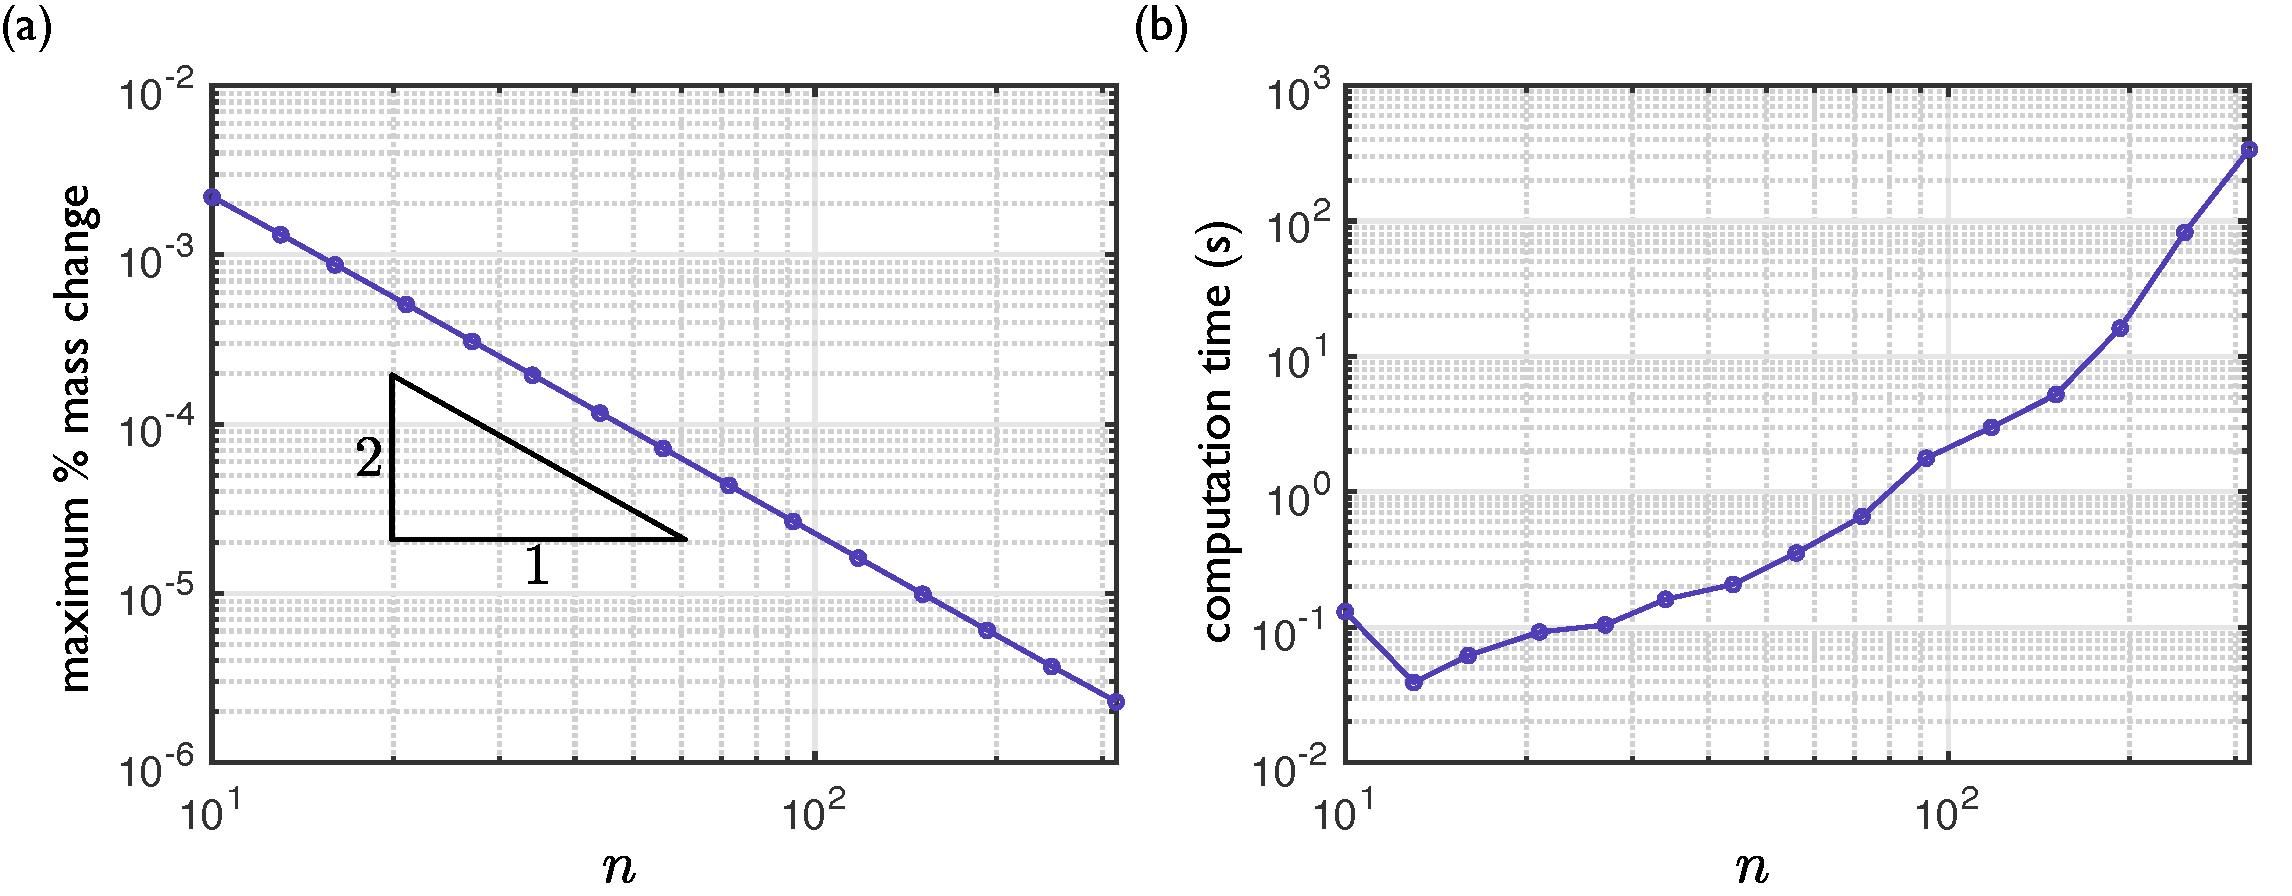
\includegraphics[width = \textwidth]{SpeedTests}
\caption{Plot of (a) $\Delta M$, the maximum percentage mass change, and (b) computation time plotted as a function of the number of grid points $n$ in numerical solutions (obtained using the method of lines) of the equations~\eqref{E:Chapter2:Model:NonDim:CombinedEq1}--\eqref{E:Chapter2:Model:NonDim:CombinedEq3},~\eqref{E:Chapter2:Model:NonDim:Kinematic}, \eqref{E:Chapter2:Model:NonDim:BCClamped}--\eqref{E:Chapter2:Model:NonDim:IC}  with $\nu = 10, V = 0.2 $ and $\xright^0 = 0.8$.}\label{fig:Ch2:Numerics:Scheme:SpeedTests}
\end{figure}


\subsection{Numerical experiments}\label{S:Ch2:Numerics:Experiments}
\begin{figure}[h!]
\centering
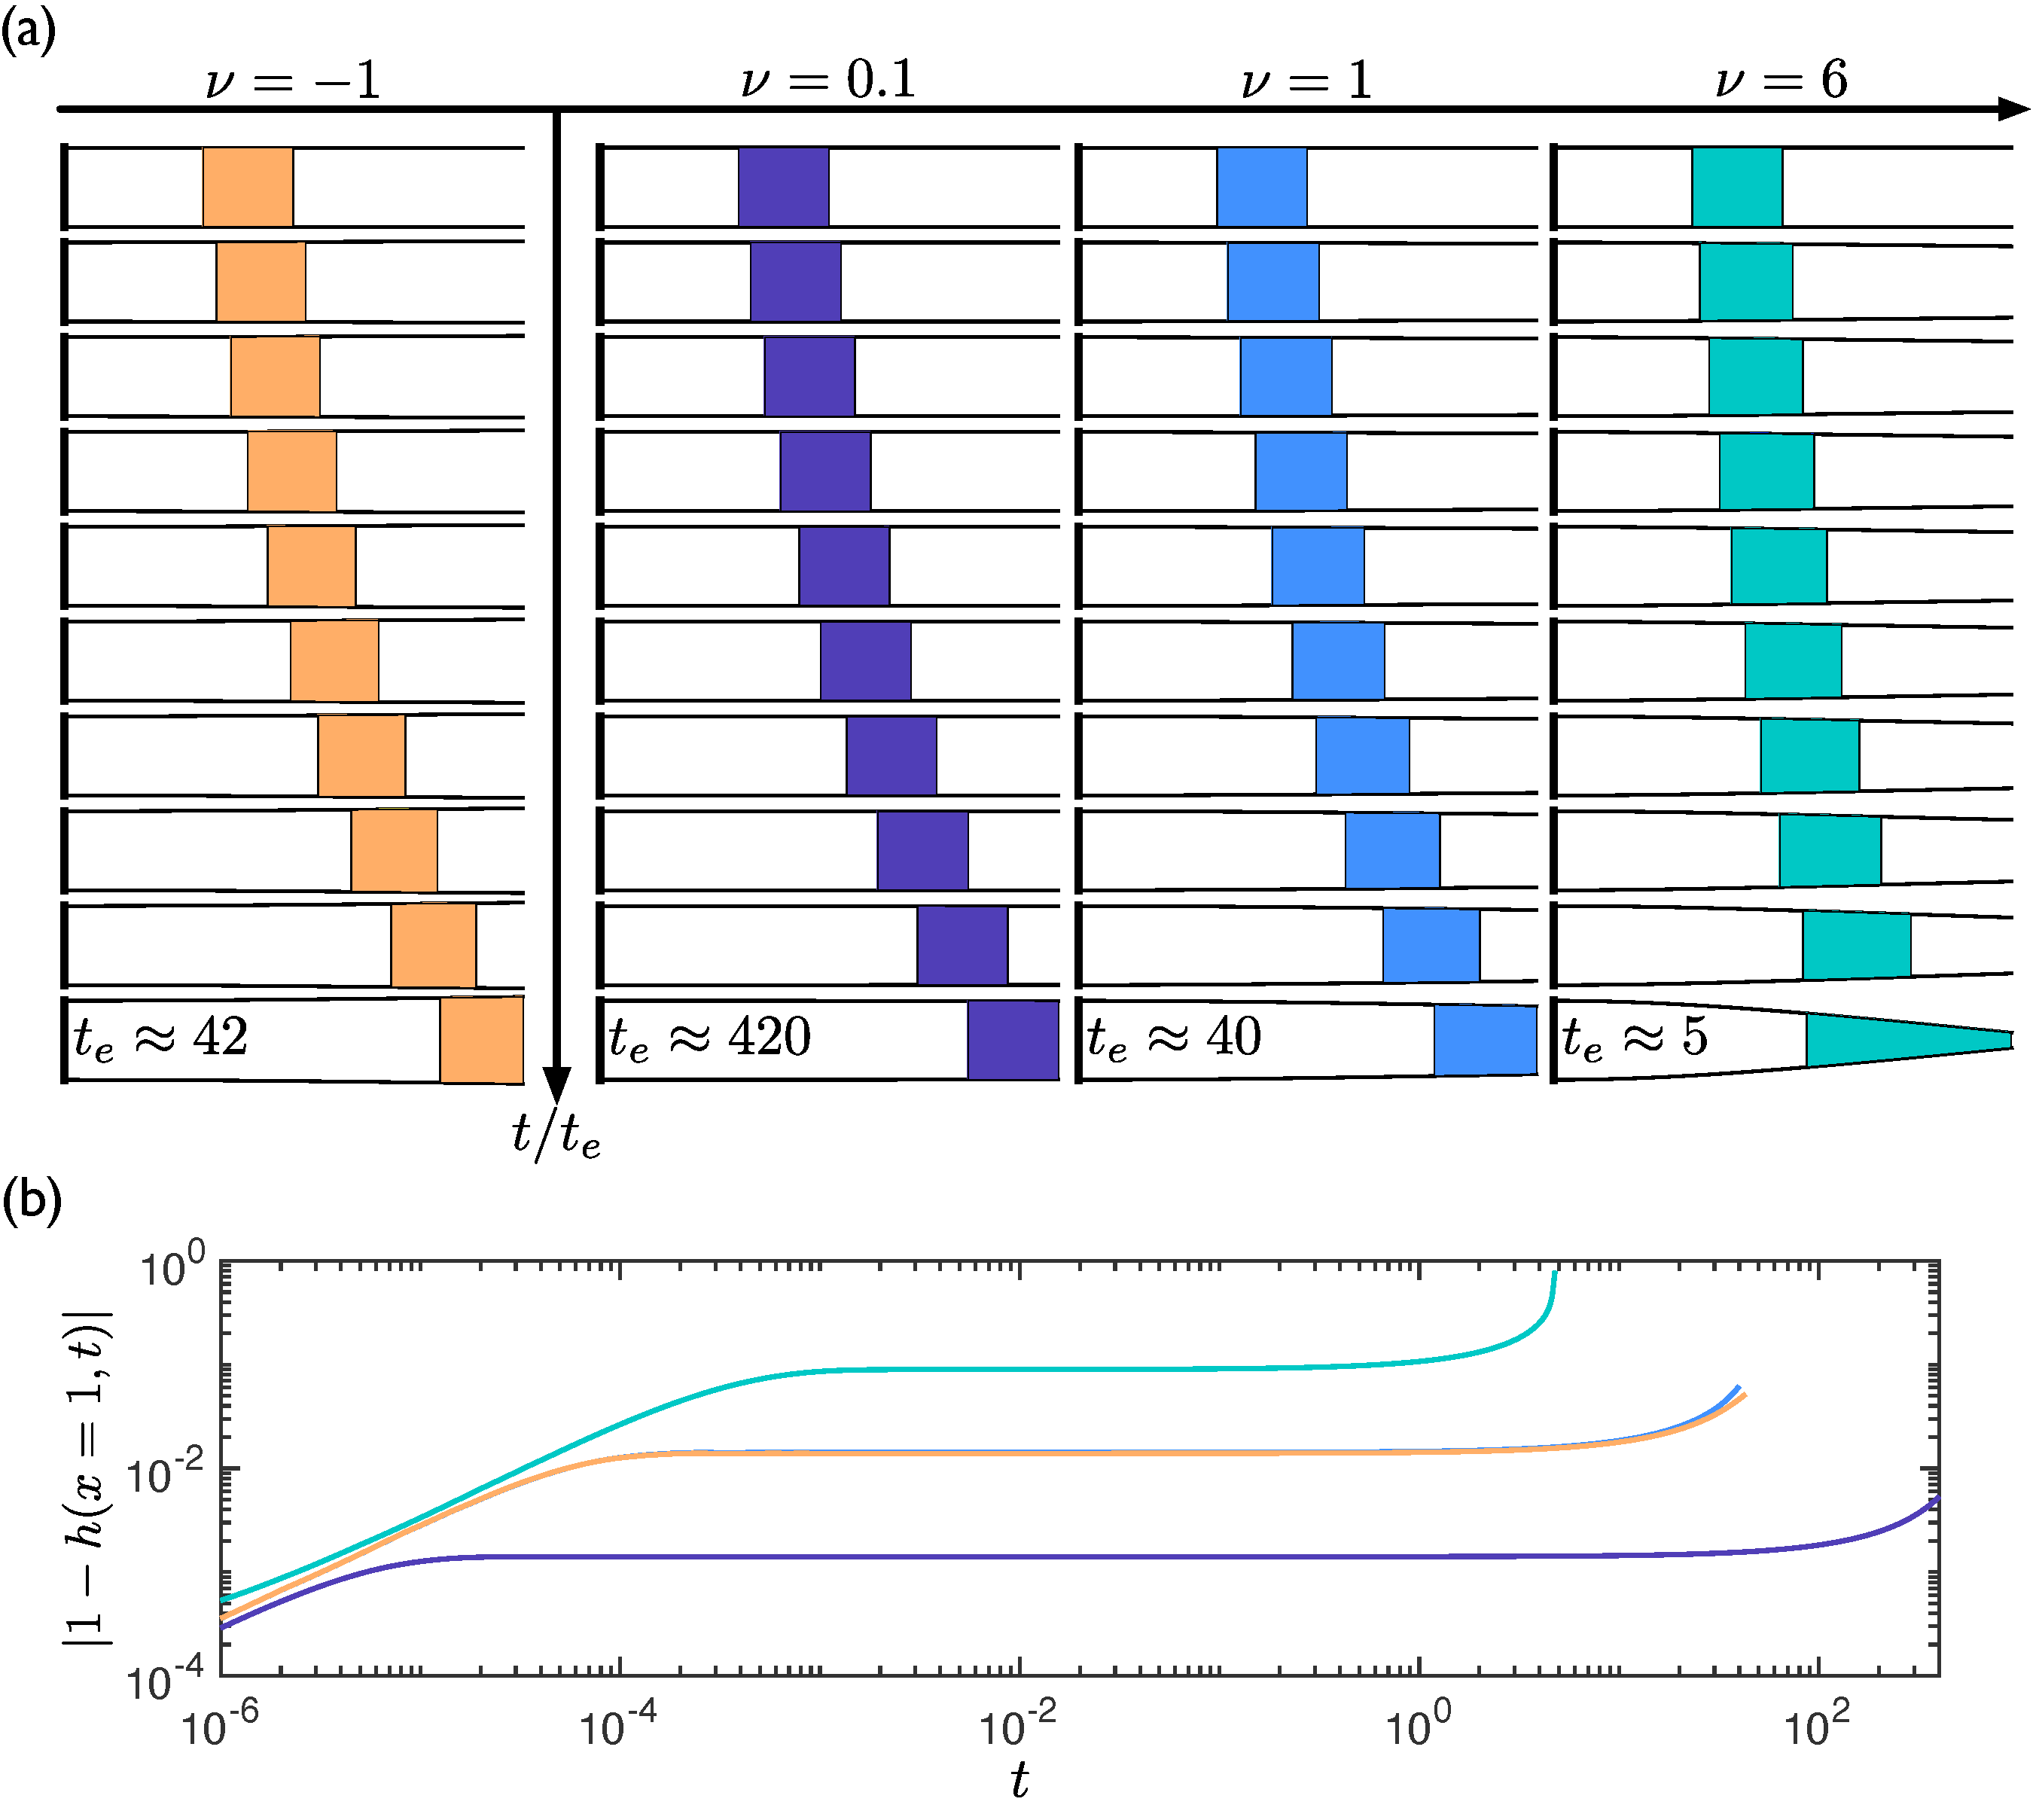
\includegraphics[width = 0.95\textwidth]{Phenomenology}
\caption{(a) Droplet-channel configurations obtained from numerical solutions of the model equations~\eqref{E:Chapter2:Model:NonDim:CombinedEq1}--\eqref{E:Chapter2:Model:NonDim:CombinedEq3},~\eqref{E:Chapter2:Model:NonDim:Kinematic}--\eqref{E:Chapter2:Model:NonDim:IC}.  The initial conditions -- $\xright^0 = 0.5, \xleft^0 = 0.3$ (giving $V = 0.2$) -- are the same for each value of $\nu$ shown. Snapshots vary linearly from $t/t_e = 0$ (top row) to $t/t_e = 1$ (bottom row), where $t_e$ denotes the time at which the droplet reaches the free end. (b) Displacement of the channel tip away from its initial position in the solutions shown in (a), with colours corresponding to those in (a). The three wetting configurations ($\nu = 0.1, 1,6$) have $h(1,t)<1$ (indicating inwards wall deflections), while the non-wetting configuration ($\nu = -1$) has $ h(1,t)>1$ (outwards deflections, respectively).}
\label{fig:Chapter2:Numerics:NumericalExperiments:Phenomenology}
\end{figure}
Schematic plots of numerical solutions of the model equations are shown in Figure~\ref{fig:Chapter2:Numerics:NumericalExperiments:Phenomenology}. The behaviour seen in these solutions span that seen in all numerical solutions; in this section, we briefly describe their features.

The salient feature of these solutions is that droplets are transported to the free end in both wetting ($\nu > 0$) and non-wetting ($\nu < 0$) scenarios, confirming that our model captures the wettability-independent nature of bendotaxis (Figure~\ref{fig:Chapter2:Numerics:NumericalExperiments:Phenomenology}(a)). Further, this droplet transport is accompanied by an inwards (outwards) deflection for wetting (non-wetting, respectively) configurations, as we predicted in our discussion of the mechanism in \S1.4.2.

In all cases, there is a qualitative similarity between the droplet trajectories, albeit on vastly different time scales (as we shall see, the droplet trajectory can be described analytically in the case of small deflections). In the proof of concept experiment, described in \S1.4.3, where $\nu = 5, \tau_c = 10$, the droplet took $\mathcal{O}(1~\text{minute})$ to traverse the channel. This is in qualitative agreement with the model result for $\nu = 6$, which predicts that the motion to takes approximately $5\tau_c$ seconds. Additionally, in the experiment, the droplet accelerates along the channel, which is in qualitative agreement with the shape of the droplet trajectories (Figure~\ref{fig:Chapter2:Numerics:NumericalExperiments:Phenomenology}(a)). (In the following chapter we describe a suite of detailed experiments designed to test the assumptions of our model -- especially the lubrication approximation within the droplet -- more closely.)

Stronger surface tension (larger $\nu$) is associated with larger deflections (Figure~\ref{fig:Chapter2:Numerics:NumericalExperiments:Phenomenology}(b)). As predicted, when surface tension is relatively strong, and the liquid wets the channel walls ($\nu = 6$ case in Figure~\ref{fig:Chapter2:Numerics:NumericalExperiments:Phenomenology}), the beam ends approach one another during the motion. As a result, the droplet spreads out, occupying a greater portion of the  length of the channel. Note that the value of $\nu = 6$ is (approximately) the largest $\nu$ for which the channel walls do not touch before the droplet reaches $\xright = 1$ (for this particular pair of initial conditions $(\xleft^0, \xright^0)$); if $\nu  \gtrsim 6$, the simulation ends before the droplet reaches $\xright = 1$, when the channel walls touch (we shall discuss what happens beyond this point in Chapter 4).

Recent studies of bendo-capillary imbibition from a bath of liquid~\citep{vanHonschoten2007JApplPhys,Aristoff2011IntJNonlinMech} have shown that the leading meniscus decelerates throughout the motion. By contrast, we observe here that droplets accelerate as they move along the channel (Figure~\ref{fig:Chapter2:Numerics:NumericalExperiments:Phenomenology}(a)). This acceleration occurs because the channel becomes more deformable the further the droplet is from the clamped end.

In the imbibition case, there is no rear meniscus, and the pressure gradient acts over a length equal to the leading meniscus position. Although meniscus advance results in a decrease in pressure at the front -- arising from additional channel deflection -- this does not overcome the additional length over which this pressure difference acts. (Note that bendo-capillary imbibition from a fixed bath is only possible for wetting configurations). In the case of bendotaxis, however, the rear meniscus is mobile, and the length over which the pressure gradient acts does not change significantly (Figure~\ref{fig:Chapter2:Numerics:NumericalExperiments:Phenomenology}(a)), allowing the increased effective deformability of the channel to dominate.

A comparison of the displacement of the channel tip from its initial position (Figure~\ref{fig:Chapter2:Numerics:NumericalExperiments:Phenomenology}(b)) suggests that the dynamic behaviour occurs on two distinct time scales: a fast, early time scale -- arising from a torque imbalance on the channel walls (the initially undeformed walls offer no resistance), and a slower time scale on which the droplets move. (This separation of time scales can be formalised in the case of small deflections.)

We also note the similarity between the tip displacement traces (Figure~\ref{fig:Chapter2:Numerics:NumericalExperiments:Phenomenology}(b)) for $\nu = \pm1$. For the majority of the motion, the deflection in these cases is relatively small, so the linearized form of the model equations are valid; as we shall see, the tip displacement and meniscus positions are symmetric in $\nu \to -\nu$ in solutions of the linearized equations. Only when deflections are significant, and non-linearities arising from the channel permeability, meniscus pressure, and conservation of mass enter, do the traces deviate from one another.  This again highlights the importance of the small deflection regime, which we turn to now.

\section{Small deflections}\label{S:Ch2:SmallDeformations}
We seek to make analytical progress by assuming that the deflections of the channel are small. Physically, small deflections are associated with weak surface tension or stiff channel walls; in our model, these two cases can be encoded by considering
\begin{equation}\label{E:Chapter2:SmallDef:Limit}
\bendability = \frac{\gamma \cos \theta_e L^4 }{B H^2} \ll 1.
\end{equation}
In this section, we therefore perform an asymptotic analysis of the model equations in the limit $\bendability \to 0$. (Note that small deflections can be also be realised by considering a small droplet volume, $V \ll 1$; we present an asymptotic analysis for $V \ll 1$  in Appendix~\ref{A:Ch2:SmallDroplets}.)

\subsection{Asymptotic expansion}
To probe the structure of  weak deviations from an undeformed configuration, $h(x,t) = 1$, we pose an expansion of the channel width in powers of $\bendability$:
\begin{equation}\label{E:Chapter2:SmallDef:Expansion}
h(x,t) = 1 + \bendability h_1(x,t) + \bendability^2 h_2(x,t) + \dots,
\end{equation}
where $h_i = \mathcal{O}(1)$ as $\bendability \to 0$.  Inserting~\eqref{E:Chapter2:SmallDef:Expansion} into the drop-only formulation of the problem problem (equations~\eqref{E:Chapter2:Numerics:SchemE:Chapter2:Reduced:EffectiveBCLower},~\eqref{E:Chapter2:Numerics:SchemE:Chapter2:Reduced:EffectiveBCUpper}--\eqref{E:Chapter2:Numerics:SchemE:Chapter2:Reduced:ReducedProblemIC}) and expanding in powers of $\bendability$ gives the PDE on the drop region as
\begin{equation}\label{E:Chapter2:SmallDef:PDE}
3|\bendability|\ddp{h_1}{t} =  \ddp{^6 h_1}{x^6} + \bendability \ddp{}{x}\left(3h_1 \ddp{^5 h_1}{x^5} + \ddp{^5 h_2}{x^5}\right),  \quad \xleft < x < \xright,
\end{equation}
correct to $\mathcal{O}(\bendability^2)$. The boundary and kinematic conditions, also correct to $\mathcal{O}(\bendability^2)$, are
\begin{align}
\ddp{^2 h_1}{x^2} - \frac{2}{\xleft^2}\left(2\xleft \ddp{h_1}{x} - 3h_1\right) + \bendability\left[ \ddp{^2 h_2}{x^2} - \frac{2}{\xleft^2}\left(2\xleft \ddp{h_2}{x} - 3h_2\right) \right] &= 0,\label{E:Chapter2:SmallDef:BC1}\\
\ddp{^3 h_1}{x^3} - \frac{6}{\xleft^3}\left(\xleft \ddp{h_1}{x} - 2h_1\right) + \bendability\left[ \ddp{^3 h_2}{x^3} - \frac{6}{\xleft^3}\left(\xleft \ddp{h_2}{x} - 2h_2\right) \right] &= 0,\label{E:Chapter2:SmallDef:BC2}\\
\ddp{^4 h_1}{x^4} + 1 + \bendability \left(\ddp{^4 h_2}{x^4} - h_1\right) &=0\label{E:Chapter2:SmallDef:BC3}
\end{align}
at $x = \xleft$,  and
\begin{align}
\ddp{^2 h_1}{x^2} + \bendability \ddp{^2 h_2}{x^2} &=0,\label{E:Chapter2:SmallDef:BC4}\\
\ddp{^3 h_1}{x^3} + \bendability \ddp{^3 h_2}{x^3} &=0,\label{E:Chapter2:SmallDef:BC5}\\
\ddp{^4 h_1}{x^4} + 1 + \bendability \left(\ddp{^4 h_2}{x^4} - h_1\right)&=0,\label{E:Chapter2:SmallDef:BC6}
\end{align}
at $x = \xright$, and
\begin{equation}\label{E:Chapter2:SmallDef:Kinematic}
3\mathrm{sgn}(\bendability) \ddp{x_{\pm}}{t} =\left. \left[  \ddp{^5 h_1}{x^5}  + \bendability \left(2 h_1 \ddp{^5 h_1}{x^5} +\ddp{^5 h_2}{x^5}\right)\right]\right|_{x = x_{\pm}}.
\end{equation}
Here $\mathrm{sgn}$ is the signum function, returning $1$ for $\nu > 0$ and $-1$ for $\nu < 0$, which arises from $\nu/|\nu| = \mathrm{sgn}(\nu)$.
\subsection{Separation of time scales}
The hierarchy of problems resulting from the asymptotic expansion sheds light on the different time scales alluded to earlier in \S\ref{S:Ch2:Numerics:Experiments}. We discuss these time scales briefly here.

By comparing the first term on the left hand side of~\eqref{E:Chapter2:SmallDef:PDE} with the first term on the right hand side, we identify a balance between channel squeezing and flux divergence on a fast ($\mathcal{O}(|\bendability|)$) time scale. Explicitly, if $T = t/|\bendability| \sim \mathcal{O}(1)$, the leading order equation in~\eqref{E:Chapter2:SmallDef:PDE} reads
\begin{equation}\label{E:Chapter2:SmallDef:TimeScales:FastPDE}
3\ddp{h_1}{T} = \ddp{^6 h_1}{x^6},
\end{equation}
and~\eqref{E:Chapter2:SmallDef:Kinematic} reads
\begin{equation}\label{E:Chapter2:SmallDef:TimeScales:FastKBC}
\ddp{x_{\pm}}{T} = \mathcal{O}(\bendability),
\end{equation}
i.e.~droplets do not move appreciably on this fast time scale. Equations~\eqref{E:Chapter2:SmallDef:TimeScales:FastPDE} and~\eqref{E:Chapter2:SmallDef:TimeScales:FastKBC} describe how the (initially straight) channel walls respond quickly to the non-zero droplet pressure by bending; this deflection induces a restoring force within the beams to balance the droplet pressure. The menisci move an $\mathcal{O}(\bendability)$ amount during this motion (in opposite directions because mass must be conserved), which is small in comparison with the total length of the channel. As it provides no information about the droplet motion, we do not pursue the problem on this time scale further.

It appears, from~\eqref{E:Chapter2:SmallDef:Kinematic}, that there is a balance between droplet motion and the leading order pressure gradient, $\partial^5 h_1/ \partial x^5$, on an $\mathcal{O}(1)$ time scale. From~\eqref{E:Chapter2:SmallDef:PDE}, we see that the leading order pressure gradient is quasistatic on this time scale: $\partial^5 h_1/ \partial x^5$ is a function of time only,  and hence the leading order pressure simply interpolates between its values at the two menisci. However, from~\eqref{E:Chapter2:SmallDef:BC3} and~\eqref{E:Chapter2:SmallDef:BC6}, these mensicus pressures are identical. Therefore the leading order pressure gradient is zero and the droplet does not move appreciably on an $\mathcal{O}(1)$ time scale either. As we shall see, the droplet moves on a long ($\mathcal{O}(|\bendability|^{-1})$) time scale; the large difference in the magnitude of this long time scale, and the short time scale on which the channel initially responds to applied pressure can be seen in our numerical solutions (see Figure~\ref{fig:Chapter2:Numerics:NumericalExperiments:Phenomenology}(b), for example).

\subsection{Droplet motion time scale}
To analyse the problem on the time scale of droplet motion, we rescale time by introducing $\tau = 3|\bendability| t \sim \mathcal{O}(1)$.  The PDE for $h_1(x,\tau)$ is
\begin{equation}\label{E:Chapter2:SmallDef:SlowTimescale:PDE}
\ddp{^6h_1}{x^6} = 0 \qquad \xleft(\tau) < x <\xright(\tau).
\end{equation}
The boundary conditions
\begin{equation}\label{E:Chapter2:SmallDef:SlowTimescale:BC1}
\ddp{^2 h_1}{x^2} - \frac{2}{\xleft^2}\left(2\xleft \ddp{h_1}{x} - 3h_1\right)= 0 = \ddp{^3 h_1}{x^3} - \frac{6}{\xleft^3}\left(\xleft \ddp{h_1}{x} - 2h_1\right) \quad \text{at}~x = \xleft,
\end{equation}
\begin{equation}\label{E:Chapter2:SmallDef:SlowTimescale:BC2}
\ddp{^2 h_1}{x^2} = 0 = \ddp{^3 h_1}{x^3}  \quad \text{at}~x = \xright, \qquad  \ddp{^4 h_1}{x^4}  = -1 \quad \text{at}~x = x_{\pm}
\end{equation}
are unaffected by the time scaling (and hence the problem for $h_1(x,\tau)$ is identical to that for $h_1(x,t)$).

The solution to~\eqref{E:Chapter2:SmallDef:SlowTimescale:PDE}--\eqref{E:Chapter2:SmallDef:SlowTimescale:BC2} is
%\begin{equation}\label{E:Chapter2:SmallDef:SlowTimescale:Solution}
%h_1(x,\tau) =-  \frac{1}{24}\left[(\xright- x)^4 - 4(\xright^3 - \xleft^3)(\xright -x) + (3\xright^4 + \xleft^4 - 4\xright \xleft^3)\right]
%\end{equation}
%\blue{equivalent and probably nicer}
%\begin{multline}\label{E:Chapter2:SmallDef:SlowTimescale:Solution}
%h_1(x,\tau) =-  \frac{\xright^4}{24}\left\{\left(1- \frac{x}{\xright}\right)^4 - 4\left[1 - \left(\frac{\xleft}{\xright}\right)^3\right]\left(1 -\frac{x}{\xright}\right) +\right.\\\left. \left[3 +\left(\frac{\xleft}{\xright}\right)^4 - 4 \left(\frac{\xleft}{\xright}\right)^3\right]\right\}
%\end{multline}
%\blue{maybe even nicer?}
\begin{equation}\label{E:Chapter2:SmallDef:SlowTimescale:Solution}
h_1(x,\tau) =-  \frac{\xright^4}{24}\left[\left(1-\xi\right)^4 - 4(1 - \xi_m^3)(1 -\xi) + (3 +\xi_m^4 - 4 \xi_m^3)\right]
\end{equation}
where $\xi(x, \tau) = x/\xright(\tau)$ and $\xi_m(\tau) = \xleft(\tau) /\xright(\tau)$. Although the deflection~\eqref{E:Chapter2:SmallDef:SlowTimescale:Solution} does not contribute to the meniscus motion (as discussed, it corresponds to a uniform pressure), it is necessary to solve for $h_1$  to determine $h_2(x, \tau)$ and thus the droplet motion via the kinematic boundary condition, which reads
\begin{equation}\label{E:Chapter2:SmallDef:SlowTimescale:Kinematic}
\dd{x_{\pm}}{\tau} = -\left.\ddp{^5 h_2}{x^5}\right|_{x = x_\pm(\tau)},
\end{equation}
at leading order.

The problem for $h_2(x, \tau)$ is also quasi-static:
\begin{equation}\label{E:Chapter2:SmallDef:SlowTimescale:PDE_firstorder}
\ddp{^6h_2}{x^6} = 0 \qquad \xleft(\tau) < x <\xright(\tau),
\end{equation}
with boundary conditions
\begin{equation}\label{E:Chapter2:SmallDef:SlowTimescale:firstorder_BC1}
\ddp{^2 h_2}{x^2} - \frac{2}{\xleft^2}\left(2\xleft \ddp{h_2}{x} - 3h_2\right)= 0 = \ddp{^3 h_2}{x^3} - \frac{6}{\xleft^3}\left(\xleft \ddp{h_2}{x} - 2h_2\right) \quad \text{at}~x = \xleft,
\end{equation}
\abeqn{E:Chapter2:SmallDef:SlowTimescale:firstorder_BC2}{\ddp{^2 h_2}{x^2} = 0 = \ddp{^3 h_2}{x^3}  \quad \text{at}~x = \xright, \qquad  \ddp{^4 h_2}{x^4}  =  h_1 \quad \text{at}~x = x_{\pm}.}
Note that the only inhomogeneity in the $h_2$ problem comes via the forcing in the pressure at $x_{\pm}$ (i.e.~through~\eqref{E:Chapter2:SmallDef:SlowTimescale:firstorder_BC2}b).

From~\eqref{E:Chapter2:SmallDef:SlowTimescale:PDE_firstorder}, we see that the pressure gradient is spatially independent, and thus set by the pressure difference across the droplet:
\begin{equation}
\ddp{^5 h_2}{x^5} = \frac{h_1(\xright,\tau) - h_1(\xleft, \tau)}{\xright - \xleft} =-\frac{\xright(\tau)^3}{8}\left[1-\xi_m(\tau)\right]\left[1+\xi_m(\tau)\right]^2.
\end{equation}
Here we have used the solution~\eqref{E:Chapter2:SmallDef:SlowTimescale:Solution} to evaluate $h_1(x_\pm,t)$. It is then clear from the kinematic condition~\eqref{E:Chapter2:SmallDef:SlowTimescale:Kinematic} that both menisci move at the same speed,
\begin{equation}\label{E:Chapter2:SmallDef:SlowTimescale:ODE}
\dd{x_{\pm}}{\tau}  = \frac{\xright^3}{8}(1-\xi_m)(1+\xi_m)^2 = \frac{(\xright - \xleft)(\xright + \xleft)^2}{8}
\end{equation}
and hence the drop length $\xright - \xleft$ does not change at leading order during the motion. Since the menisci do not move appreciably on the faster time scales discussed above (recall that on an $\mathcal{O}(|\bendability|^{-1})$ time scale the menisci move an $\mathcal{O}(\bendability)$ amount), the droplet length stays at its initial value, $\xright - \xleft\approx  \xright^0 - \xleft^0 = V$ and thus $\xright + \xleft \approx 2\xright - V$.

Using this, the solution to~\eqref{E:Chapter2:SmallDef:SlowTimescale:ODE} with initial condition $\xright(\tau = 0) =\xright(t = 0) = \xright^0$, is, in terms of the original (unscaled) dimensionless variables,
\begin{equation}\label{E:Chapter2:SmallDef:SlowTimescale:xright_original_variables}
\xright(t) = \frac{V}{2}\left[1 + \left(\frac{V}{2\xright^0 - V} - \frac{3V^2 |\bendability | t}{4}\right)^{-1}\right] + \mathcal{O}(|\bendability|^2),
\end{equation}
with $\xleft = \xright - V + \mathcal{O}(|\bendability|)$. Note that  this expression is symmetric in $\nu \rightarrow -\nu$: droplets in channels with the same absolute bendability, but with different wettability conditions, travel at the same speed when the channel deflections are small, as observed in numerical solutions presented in \S\ref{S:Ch2:Numerics:Experiments}.


\begin{figure}[th]
\centering
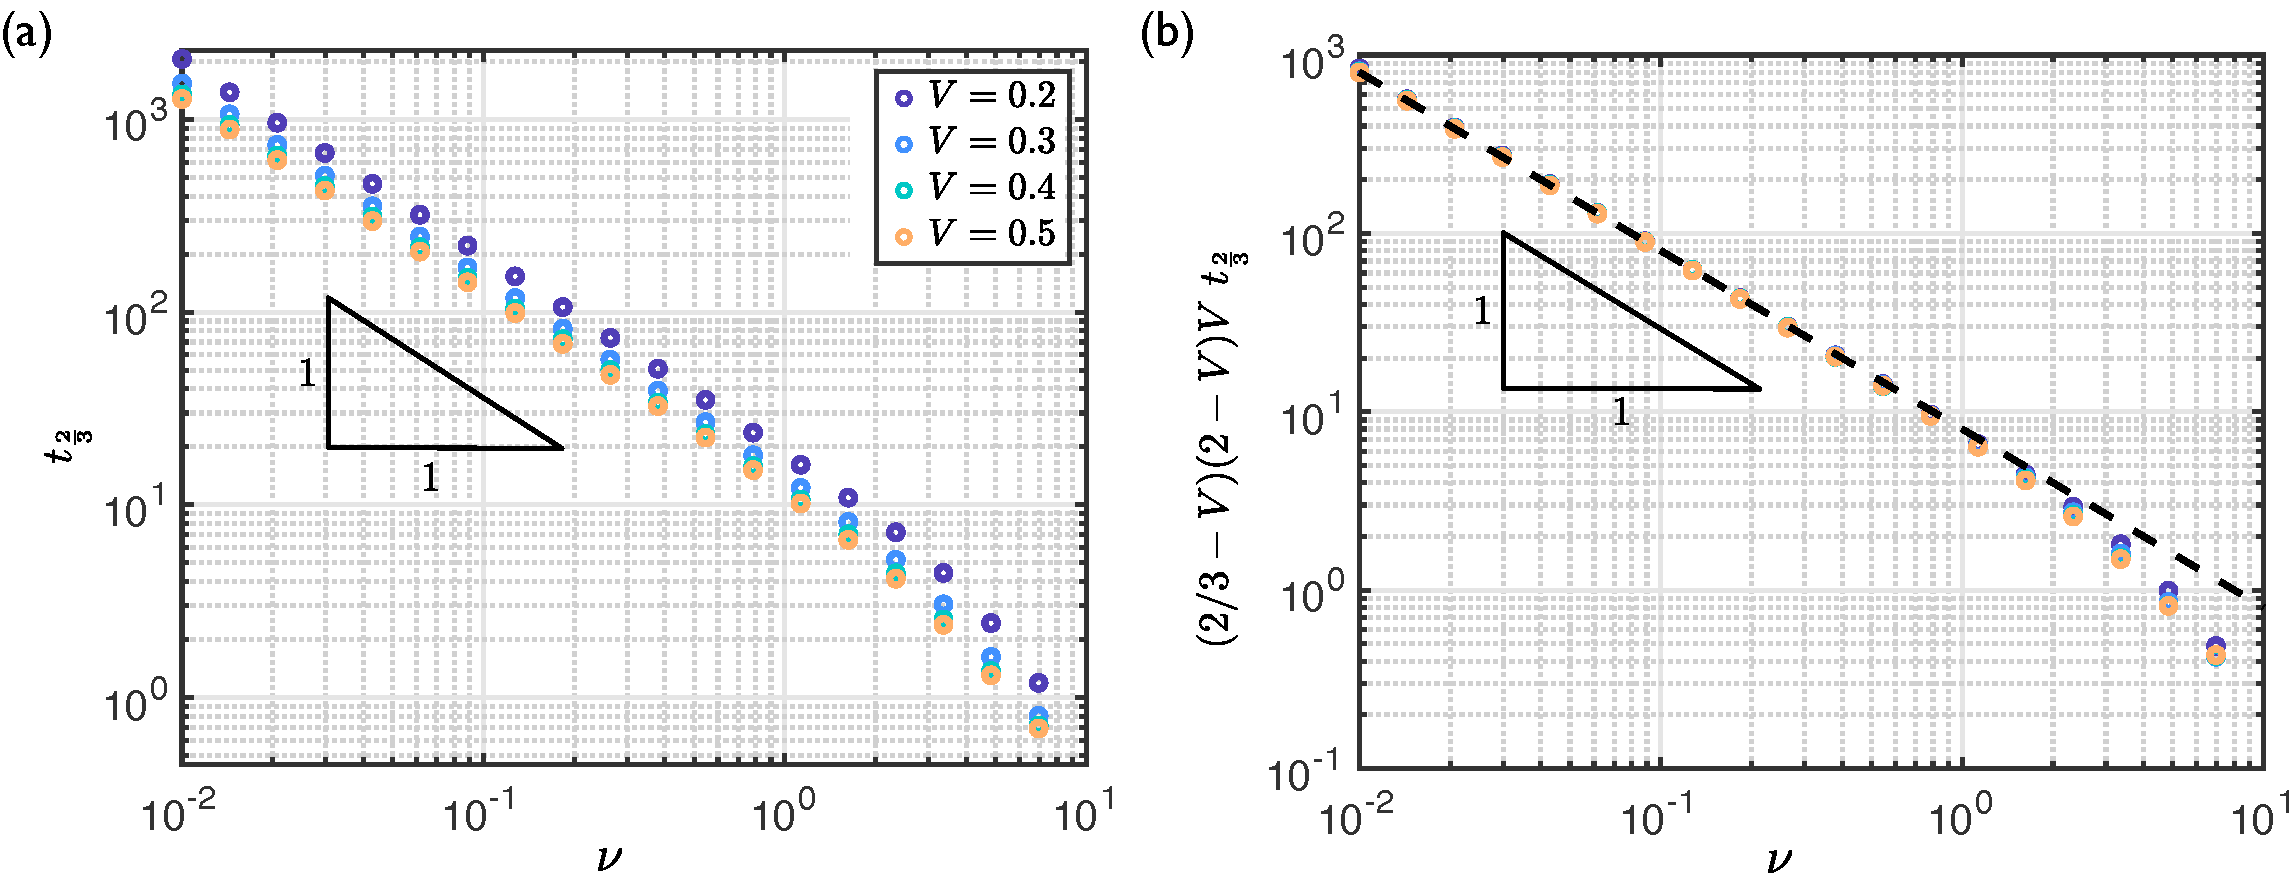
\includegraphics[width = \textwidth]{Asymptotics}
\caption{(a) Numerically obtained values of $t_{2/3}$ (the time taken for the droplet to traverse the last 1/3\textsuperscript{rd} on the channel) plotted on logarithmic axes. The colour of points indicates the relative volume $V$ (see legend in (a)). (b) Data in (a) rescaled according to the asymptotic prediction~\eqref{E:Chapter2:SmallDef:SlowTimescale:AsymptoticTf}. The dashed black line indicates $t_{2/3} = t_{2/3}^{\text{SB}}$, the asymptotic result in the case of small deflections.}
\label{fig:Chapter2:SmallDeformations:Asymptotics}
\end{figure}

As a proxy for the time scale of motion, we consider $t_f$ -- the time taken for the leading meniscus to pass from $\xright = f < 1$ to the free end, $\xright = 1$. As $t_f$ is the time \emph{difference} between two events, the system is free of inertia, and the capillary torque is balanced by beam bending (except for at early times, when the droplet does not move significantly), we expect $t_f$ to be approximately independent of the initial conditions. This allows us to consider the dynamic behaviour only in terms of the control parameters of interest: $\bendability$ and $V$. (As we shall see, $t_f$, rather than the total time for the motion, is the relevant observable  in our experimental study of bendotaxis.)

Using the solution~\eqref{E:Chapter2:SmallDef:SlowTimescale:xright_original_variables}, we find that the small bendability estimate of $t_f$, denoted $t_f^\text{SB}$, is
\begin{equation}\label{E:Chapter2:SmallDef:SlowTimescale:AsymptoticTf}
t_f^{\text{SB}} = \frac{24(1 - f)}{(2f - V)(2 - V)}\frac{1}{|\nu| V},
\end{equation}
Noting that
\begin{equation}\label{E:Chapter2:SmallDef:SlowTimescale:ComparisonToScaling}
\frac{1}{\nu V} =  \frac{B H^2}{|\gamma \cos \theta_e| L^4}\frac{L}{\Delta X}  =  \frac{B}{|\gamma \cos \theta_e| \Delta X}\frac{H^2}{L^3},
\end{equation}
the result~\eqref{E:Chapter2:SmallDef:SlowTimescale:AsymptoticTf} is in agreement with the result of the scaling argument presented in \S\ref{S:Model:Scaling}, namely equation~\eqref{E:Chapter2:Model:Scaling:ScalingResult}.

Numerical solutions of the full problem with $\nu \ll 1$ agree well with~\eqref{E:Chapter2:SmallDef:SlowTimescale:AsymptoticTf} (Figure~\ref{fig:Chapter2:SmallDeformations:Asymptotics}). These results are shown for $t = t_f$ with $f = 2/3$ (in which case $t_f$ is the time taken to traverse the final 1/3\textsuperscript{rd} of the channel). Surprisingly, the expression~\eqref{E:Chapter2:SmallDef:SlowTimescale:AsymptoticTf} accurately predicts $t_f$ in numerical solutions even when $\nu = \mathcal{O}(1)$, and the asymptotic analysis is no longer valid.

To understand this, we consider the dynamics in the limit of small droplets ($V \ll 1$): in Appendix~\ref{A:Ch2:SmallDroplets}, we show that the corresponding small droplet result for $t_f$ is
\begin{equation}\label{E:Chapter2:SmallDef:SlowTimescale:AsymptoticTfSmallVolume} t_f^{\text{SV}} = \frac{6(1 - f)}{f}\frac{1}{|\nu| V},
\end{equation}
Note that
\begin{equation}
\frac{24(1 - f)}{(2f - V)(2 - V)} =  \frac{6(1 - f)}{f}\left[1 + \frac{V^2}{4f} + \mathcal{O}(V)\right],
\end{equation}
i.e.~$t_f^{\text{SB}} = t_f^{\text{SV}} + \mathcal{O}(V)$. The agreement between numerical solutions and~\eqref{E:Chapter2:SmallDef:SlowTimescale:AsymptoticTf}  for $\nu = \mathcal{O}(1)$ (Figure~\ref{fig:Chapter2:SmallDeformations:Asymptotics}) in fact reflects agreement with the result~\eqref{E:Chapter2:SmallDef:SlowTimescale:AsymptoticTfSmallVolume} for small volumes. As mentioned, both the cases of small bendability (and $V \lesssim \mathcal{O}(1)$) and small droplet volume (and $\nu \lesssim \mathcal{O}(1)$) will result in a small channel deflections, but the asymptotic analysis of this section is only valid in the case of the former. Note that, the larger $V$ is, the sooner the data from numerical solutions `peel off' from the asymptotic result~\eqref{E:Chapter2:SmallDef:SlowTimescale:AsymptoticTf}~(Figure~\ref{fig:Chapter2:SmallDeformations:Asymptotics}(b)). It is difficult to separate the two small deflections cases -- small bendability and small droplet volume -- since droplets have $V < 1$ by construction (and we are typically interested in $V < 1/2$).


\section{Droplet removal}
\begin{figure}
\centering
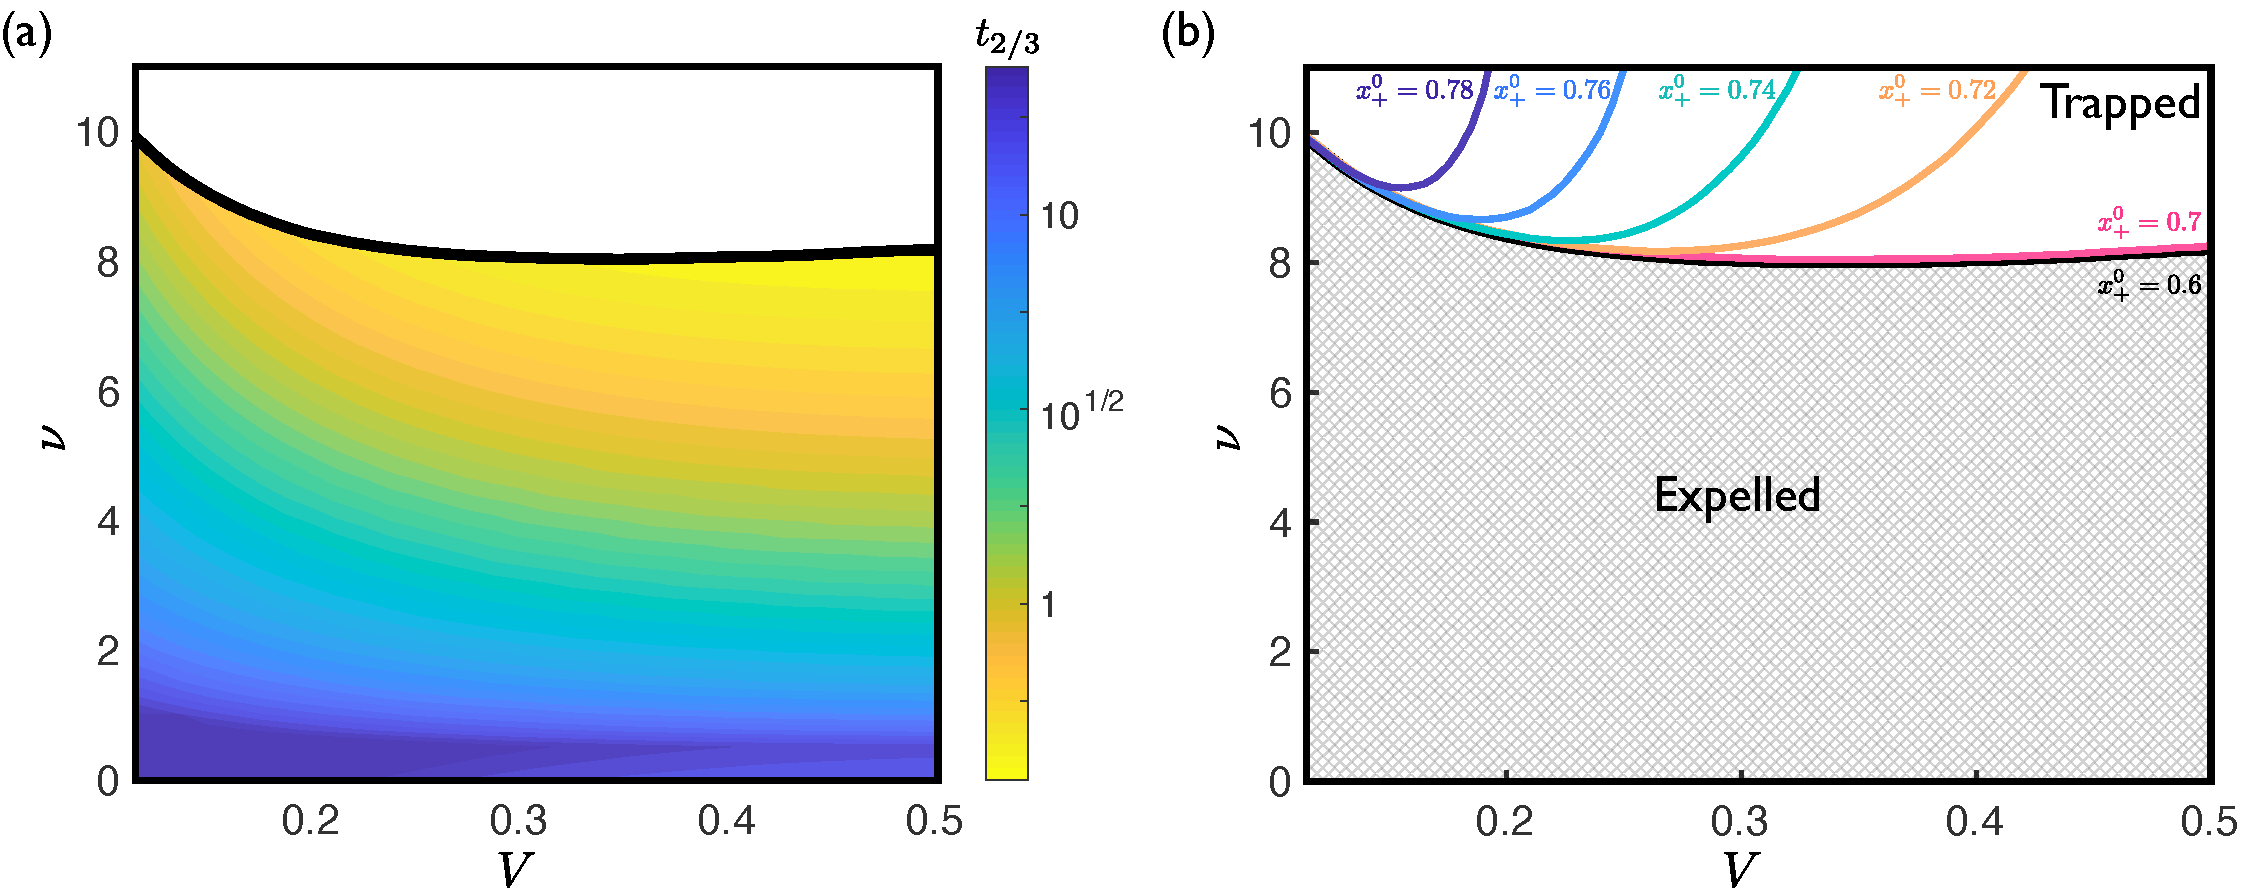
\includegraphics[width = 0.95\textwidth]{optimal_removal_split}
\caption{(a) Influence of dimensionless droplet volume $V$ and channel bendability $\nu$ on numerically obtained values of $t_{2/3}$ (the time taken to traverse the final 1/3\textsuperscript{rd} of the channel) with $\xright^0 = 0.6$. The solid black line indicates indicates $\nu_c(V,\xright^0 = 0.6)$, the smallest value of $\nu$ (for a given $V$) in which the channel walls touch before the droplet reaches the free end. (b) Numerically obtained values of $\nu_c(V,\xright^0)$ for different initial droplet positions $\xright^0$. Droplets are always expelled (reach the free end) for $\nu < \nu_c$, and trapped (the channel walls touch before the droplet reaches the free end) for $\nu > \nu_c$ (the hatched region indicates the expelled region for $\xright^0 \lesssim 0.7$).}
\label{fig:Ch2:DropRemoval}
\end{figure}
We conclude this chapter with a brief discussion of the implications of our model for droplet removal from deformable channels --  our main motivation for studying bendotaxis. In particular, we consider the time taken for a droplet to reach the free end (from which it can be removed). This quantity is important because the overall performance of the structure is strongly dependent on the number of compromised channels -- those containing a droplet. Increasing the speed of removal from individual channels will minimise the total number of compromised channels.

A key question is, therefore, how should a channel be designed to minimize the time taken for droplets to reach the free end? In answering this question, we again consider $t_f$, rather than the total time taken, to isolate the effects of the bendability $\nu$ and droplet volume $V$.

We solve the model equations presented in \S\ref{S:Chapter2:Model:NonDim} numerically for a variety of $(V, \nu)$ pairs to map $t_f$ as a function of $\nu$ and $V$ (Figure~\ref{fig:Ch2:DropRemoval}(a)). This map confirms the trend suggested by those numerical solutions shown in Figure~\ref{fig:Chapter2:Numerics:NumericalExperiments:Phenomenology}: increasing the  bendability, $\nu = \gamma \cos \theta_e L^4/(BH^2)$, reduces the time taken for the droplets to traverse a section of the channel adjacent to the free end. However, this is to be weighed against the possibility that the walls touch during the motion and trap (wetting) drops indefinitely. The regions of $(V, \nu)$ space for which the droplet is ultimately trapped or reaches the free end is shown in Figure~\ref{fig:Ch2:DropRemoval}(b). %some m ention of (a) how this is acheived in practice (e.g. lengthening channel), (b) the hidden L^2/H_0 in the time scale?

We denote by $\nu_c(V,\xright^0)$ the smallest value of $\nu$ at which the channel walls touch -- and trap the drop -- during the motion (before $t = t_e$, when the simulation ends), for a given  droplet volume $V$ and initial position $\xright^0$, i.e.
\begin{equation}
\nu_c = \sup\left\{\nu | h(x = 1, t = t_e) > 0\right\}.
\end{equation}
(This supremum is well defined because $h(x = 1, t = t_e)$ is a decreasing function of $\nu$ for a given $(V, \xright)$.) We compute $\nu_c$ numerically using a bisection scheme. Each evaluation of $h(x = 1, t = t_{e})$ requires us to solve the model equations numerically for $t \leq t_e$.

We plot in Figure~\ref{fig:Ch2:DropRemoval}(b) the curves $\nu_c$ as a function of $V$, for various $\xright^0$.These curves are approximately independent of $\xright^0$ when $\xright^0 \lesssim 0.7$, but are very sensitive to $\xright$ when $\xright^0>0.7$ (i.e.~$\partial \nu_c /\partial \xright^0 \gg 1$ when $\xright^0>0.7$). To understand this we note that, provided the channel walls do not touch, the channel width at $x = 1$ depends only on the channel width and slope at $x = \xright$, and the (instantaneous) droplet position via the distance $1 - \xright$ between the channel end and the `$+$' meniscus (see equation~\eqref{E:Chapter2:Numerics:SchemE:Chapter2:Reduced:ShapeUpper}).  In general, the channel width and slope are set by an instantaneous torque balance on the beams, and the history of the droplet is unimportant. This torque balance is, however, not valid during the early squeezing regime: droplets starting close to the free end may be able to reach it during this period. For a given $V$, a stronger pull (larger $\nu$) is required to trap those droplets starting close to the free end.

\section{Summary}
In this section, we have developed a mathematical model of bendotaxis. The physics retained in our model is motivated by the experimental demonstration of bendotaxis presented in \S1.4.3. The model is characterized by three dimensionless parameters: a channel bendability (which implicitly describes the wettability conditions), a dimensionless droplet volume and a dimensionless starting position of the droplet.

Numerical solutions of the governing equations indicate that our model captures the wettability independent nature of bendotaxis, and its characteristic inwards deflections for wetting configurations and outwards deflection for non-wetting configurations. The numerical solutions predict motion on a time scale comparable to the experimental demonstration, with qualitatively similar dynamics. However, we have not made a detailed quantitative comparison between this experiment and the model; in the following chapter, we describe a suite of experiments similar to the proof of concept experiment which are designed to test the validity of our model.

We demonstrated how analytic progress can be made in quantifying the time scale of motion in the case of small deflections -- achieved by having either a small channel bendability or a small droplet volume. In both cases, the time scale of motion is inversely proportional to the product of the bendability and droplet volume, as was also predicted by a scaling argument. We also discussed the implications of our model for droplet removal from deformable channels; in particular, we identified that high channel bendability is desirable for quick droplet removal, but this this is to be weighed against the possibility of the tips of the channel walls touching and trapping wetting drops indefinitely. Finally, we note that for $\nu \lesssim 8$, droplets are always expelled, regardless of where the start in the channel; tailoring the surfaces design to ensure $\nu \lesssim 8$ may therefore be a good design criterion for superhydrophobic surfaces that exploit bendotaxis for anti-fogging.


%%%%%%%%%%%%%%%%%Appendices%%%%%%%%%%%%%%%
% uncomment below for thesis main compile
\begin{subappendices}
%\addcontentsline{toc}{section}{Appendices}
\renewcommand{\thesection}{\Alph{section}}
%\appendix
\section{Small droplets}\label{A:Ch2:SmallDroplets}
In this appendix, we consider the small volume droplets, $V \ll 1$. The aim is to derive a small volume approximation for $t_f$ -- the time taken between $\xright = f$ and $\xright = 1$ --  which we denote $t_f^{\text{SV}}$. Here we simply describe the leading order behaviour, as this is sufficient to determine $t_f^{\text{SV}}$ to leading order. %in constrast to the $\nu \ll 1$ case
\subsection{Small volume expansion}\label{A:Ch2:SmallDroplets:SmallVolumeExpansion}
We begin by assuming that the channel is not deflected significantly by the droplet, allowing us to write
\begin{equation}\label{A:E:Ch2:SmallDroplets:Expansion}
h(x,t) = 1 + Vh_1(x,t) + \mathcal{O}(V^2),
\end{equation}
where $h_1 \sim \mathcal{O}(1)$; as we shall see, enforcing this condition places a restriction on the range of $\nu$ allowed.

To begin, we first note that conservation of mass requires the length of the drop to remain small and approximately constant throughout the motion, $\xright - \xleft = V + \mathcal{O}(V^2)$.

Recall that the channel width in the drop region satisfies
\begin{equation}\label{A:E:Ch2:SmallDroplets:Reynolds}
\ddp{h}{t} = \frac{1}{3|\bendability|}\ddp{}{x}\left(h^3 \ddp{^5  h}{x^5}\right), \qquad \xleft < x <\xright.
\end{equation}
Inserting~\eqref{A:E:Ch2:SmallDroplets:Expansion} into~\eqref{A:E:Ch2:SmallDroplets:Reynolds} and integrating across the droplet gives
\begin{equation}\label{A:E:Ch2:SmallDroplets:IntegratedReynolds}
\left[h^3 \ddp{^5 h}{x^5}\right]_{\xleft}^{\xright} =3|\bendability| \int_{\xleft}^{\xright} V\ddp{h_1}{t}~\mathrm{d}x = \mathcal{O}(V^2),
\end{equation}
where the second equality makes use of the short length of the droplet. Equation~\eqref{A:E:Ch2:SmallDroplets:IntegratedReynolds} indicates that the liquid flux, which is proportional to $h^3 \partial^5h/\partial x^5$, does not vary significantly across the droplet. As a consequence, the pressure gradient is approximately (spatially) constant in the drop. Using the dimensionless Laplace pressure boundary condition~\eqref{E:Chapter2:Model:NonDim:BCPressure}, we can approximate this constant pressure gradient by
\begin{equation}\label{A:E:Ch2:SmallDroplets:DropPressureGradient}
\ddp{^5 h}{x^5} = \frac{1}{\xright - \xleft}\left[\ddp{^4 h}{x^4}\right]_{\xleft}^{\xright} + \mathcal{O}(V^2) =\frac{\nu}{\xright - \xleft}\left[\frac{1}{h(\xleft,t)} - \frac{1}{h(\xright,t)}\right] + \mathcal{O}(V^2).
\end{equation}
Now, by expanding the terms on the right hand side of~\eqref{A:E:Ch2:SmallDroplets:DropPressureGradient} as
\begin{equation}\label{A:E:Ch2:SmallDroplets:DropPressureChange}
\frac{1}{h(\xleft,t)} - \frac{1}{h(\xright,t)}  =V\left. \ddp{h}{x}\right|_{x = \xright} + \mathcal{O}(V^3) = \left.V^2 \ddp{h_1}{x}\right|_{x = \xright} + \mathcal{O}(V^3),
\end{equation}
we can express the pressure gradient as
\begin{equation}\label{A:E:Ch2:SmallDroplets:DropPressureGradient2}
\ddp{^5 h}{x^5} =\left. \nu V \ddp{h_1}{x}\right|_{x =\xright}+ \mathcal{O}(V^2),
\end{equation}
Inserting~\eqref{A:E:Ch2:SmallDroplets:DropPressureGradient2} into the kinematic condition~\eqref{E:Chapter2:Model:NonDim:Kinematic} gives (to leading order),
\begin{equation}\label{A:E:Ch2:SmallDroplets:ReducedKinematic}
\dd{\xright}{t} = -\left.\frac{\mathrm{sgn}(\nu)}{3} V\ddp{h_1}{x}\right|_{x =\xright}.
\end{equation}

\subsection{Point force problem}
To proceed, we require an estimate of the slope of the channel walls. Since the drop is small, its effect on the channel shape may be approximated by a point force acting at $x = \xright$; the channel `sees' the droplet only via jump conditions, which we derive by integrating the pressure across the droplet.

To begin, we note that, since the pressure gradient within the droplet is $\mathcal{O}(V)$ (equation~\eqref{A:E:Ch2:SmallDroplets:DropPressureGradient2}), the droplet pressure is approximately constant:
\begin{equation}\label{A:E:Ch2:SmallDroplets:DropPressure}
p(x,t) = \ddp{^4 h}{x^4} =  \left.\ddp{^4 h}{x^4}\right|_{x = \xright} + \mathcal{O}(V^2) = -\nu + \mathcal{O}(V^2)
\end{equation}
By integrating~\eqref{A:E:Ch2:SmallDroplets:DropPressure} across the droplet, we calculate the jump in shear force across it as
\begin{equation}\label{A:E:Ch2:SmallDroplets:ShearJump}
\left[\ddp{^3 h}{x^3}\right]_{\xleft}^{\xright} = -\nu V + \mathcal{O}(V^2).
\end{equation}
This is the first jump condition. The second jump condition comes from expanding the jump in channel shape across the droplet in $V$:
\begin{align}
\left[h\right]_{\xleft}^{\xright} &= h(\xright,t) - h(\xright - V,t)  \nonumber\\
&= 1 + V h_1(\xright,t) - \left[1 + V h_1(\xright - V,t)\right] + \mathcal{O}(V^2) \nonumber \\ &= 1 + V h_1(\xright,t) - \left[1 + V h_1(\xright,t)\right]+ \mathcal{O}(V^2)\nonumber \\&=  \mathcal{O}(V^2). \label{A:E:Ch2:SmallDroplets:ShapeSmall}
\end{align}

Similarly, by expanding the channel slope and moment, we obtain
\begin{equation}\label{A:E:Ch2:SmallDroplets:Slope_and_moment_small}
\left[\ddp{h}{x}\right]_{\xleft}^{\xright} = V\left.\ddp{^2 h}{x^2}\right|_{x = \xright} + \mathcal{O}(V^2), \qquad \left[\ddp{^2 h}{x^2}\right]_{\xleft}^{\xright} = V\left.\ddp{^3 h}{x^3}\right|_{x = \xright} + \mathcal{O}(V^2).
\end{equation}

Recall from \S\ref{S:Ch2:Numerics:Scheme:ReducedProblem} that the free boundary conditions applied at $x = 1$ also apply at $x = \xright$, i.e.
\begin{equation}\label{A:E:Ch2:SmallDroplets:EffFreeBC}{\left.\ddp{^2 h}{x^2}\right|_{x = \xright} = 0, \qquad \left.\ddp{^3 h}{x^3}\right|_{x = \xright} =0.}
\end{equation}
Combining~\eqref{A:E:Ch2:SmallDroplets:Slope_and_moment_small} and~\eqref{A:E:Ch2:SmallDroplets:EffFreeBC} yields the final two jump conditions
\begin{equation}\label{A:E:Ch2:SmallDroplets:Slope_and_moment_jump_conds}
\left[\ddp{h}{x}\right]_{\xleft}^{\xright} = \mathcal{O}(V^2), \qquad \left[\ddp{^2 h}{x^2}\right]_{\xleft}^{\xright} = \mathcal{O}(V^2).
\end{equation}

The leading order `point force problem' for $h_1$ is therefore
\begin{equation}\label{A:E:Ch2:SmallDroplets:PtForcePDE}
\ddp{^4 h_1}{x^4} = 0, \qquad \text{in}~0< x < \xright,~\text{and}~\xright < x < 1,
\end{equation}
with jump conditions
\begin{equation}\label{A:E:Ch2:SmallDroplets:PtForceJump}
\left[\ddp{^3 h_1}{x^3}\right]_{\xright^-}^{\xright^+} = -\nu, \qquad \left[\ddp{^2 h_1}{x^2}\right]_{\xright^-}^{\xright^+} =0, \qquad \left[\ddp{ h_1}{x}\right]_{\xright^-}^{\xright^+} =0,\qquad \left[h_1\right]_{\xright^-}^{\xright^+} = 0,
\end{equation}
and boundary conditions
\begin{align}
h_1 &= 0, \qquad  \ddp{h_1}{x}= 0, \qquad\text{at}~x = 0,\label{A:E:Ch2:SmallDroplets:PtForceBC1}\\
\dd{^2 h_1}{x^2} &= 0, \qquad \ddp{^3 h_1}{x^3}= 0, ~~\quad \text{at}~x = 1.\label{A:E:Ch2:SmallDroplets:PtForceBC2}
\end{align}
The solution to~\eqref{A:E:Ch2:SmallDroplets:PtForcePDE}--\eqref{A:E:Ch2:SmallDroplets:PtForceBC2} is
\begin{equation}\label{A:E:Ch2:SmallDroplets:SolutionShape}
h_1(x,t) = \begin{cases}{}
        -\frac{\bendability}{6}(3\xright x^2 - x^3) & \text{for }\quad 0 < x < \xright(t), \\
       -\frac{\bendability}{6}\left[3\xright^2(x - \xright) + 2 \xright^3\right] & \text{for }\quad \xright(t) < x < 1.
        \end{cases}
\end{equation}
This solution demonstrates that our assumption that $h_1\sim \mathcal{O}(1)$ is valid only when $\nu  \sim \mathcal{O}(1)$.

After inserting~\eqref{A:E:Ch2:SmallDroplets:SolutionShape} into the reduced kinematic condition~\eqref{A:E:Ch2:SmallDroplets:ReducedKinematic}, we obtain an ordinary differential equation for the meniscus position:
\begin{equation}\label{A:E:Ch2:SmallDroplets:xrightODE}
\dd{\xright}{t} = \frac{|\bendability| V \xright^2}{6}.
\end{equation}
The solution to~\eqref{A:E:Ch2:SmallDroplets:xrightODE}, with initial condition $\xright(0) = \xright^0$, is
\begin{equation}\label{A:E:Ch2:SmallDroplets:SolutionMeniscusPos}
\xright(t) = \frac{6\xright^0}{6 - |\bendability| V \xright^0 t}.
\end{equation}
Using the solution~\eqref{A:E:Ch2:SmallDroplets:SolutionMeniscusPos}, we find that the small volume estimate of $t_f$ is
\begin{equation}\label{A:E:Ch2:SmallDroplets:Solutiontf}
t_f^{\text{SV}}= \frac{6(1-f)}{|\bendability|V f}.
\end{equation}
In Figure~\ref{A:fig:Ch2:SmallDroplets}, we plot trajectories for $\xright(t)$ against $Vt$ as well as numerically obtained values of $\nu t_{2/3}$ against $V$ for several different values of $\nu$. We see that these numerically obtained values agree with the asymptotic results~\eqref{A:E:Ch2:SmallDroplets:SolutionMeniscusPos} and~\eqref{A:E:Ch2:SmallDroplets:Solutiontf}, respectively, in the limit $V \to 0$.

It is interesting to note that the numerically obtained data `over-shoots' the asymptotic result as the bendability $\nu$ decreases. The competition between the non-linearities in the Laplace pressure condition -- which tends to speed up the motion, relative to the behaviour in the limit $V \ll 1$ --  and the channel permeability -- which tends to slow the motion -- is responsible for this. For the larger values of $\nu$ shown in Figure~\ref{A:fig:Ch2:SmallDroplets}(b), the former dominates, and the motion is faster than the asymptotic result (and vice versa for the smaller values of $\nu$). (The $\nu = 3$ curve in Figure~\ref{A:fig:Ch2:SmallDroplets}(b) corresponds to these two non-linearities cancelling one another out, giving the impression of agreement with~\eqref{A:E:Ch2:SmallDroplets:Solutiontf} for $V\sim \mathcal{O}(1)$.)

\begin{figure}[t]
\centering
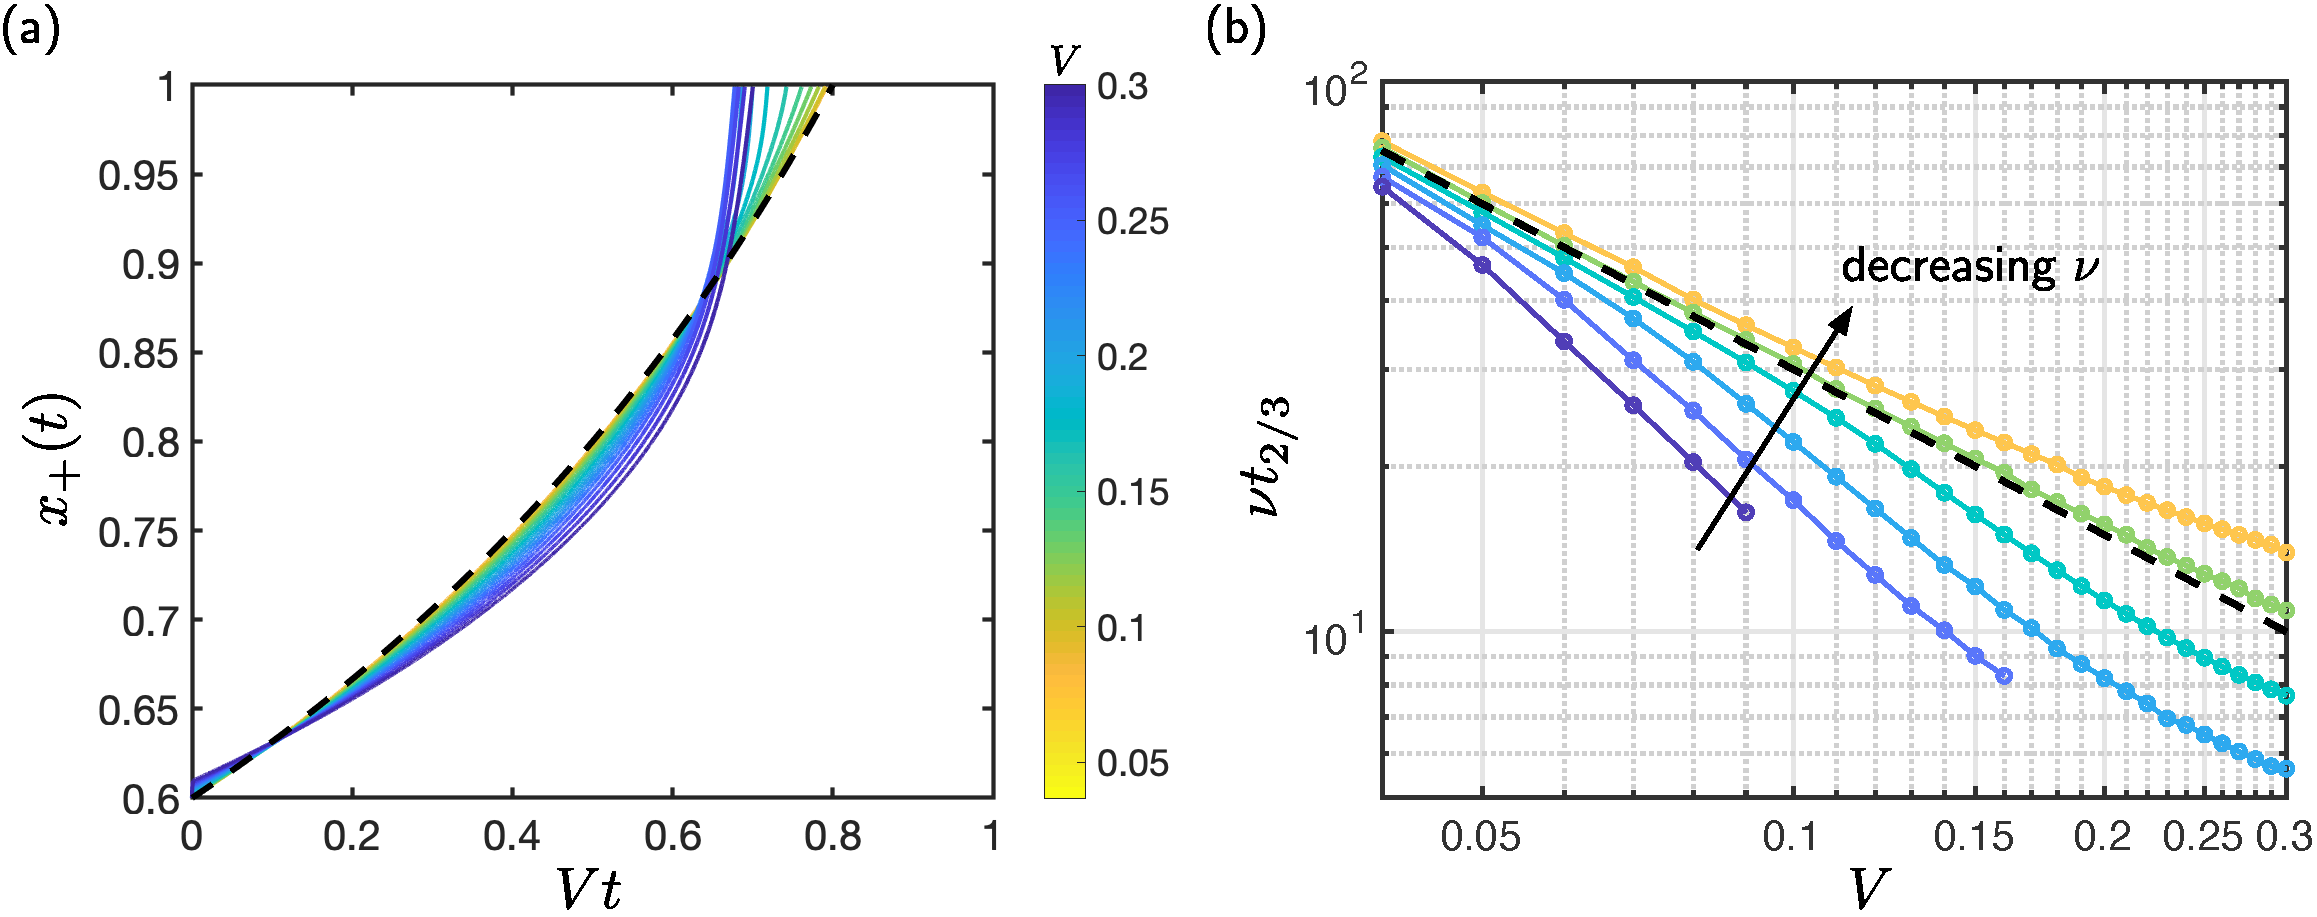
\includegraphics[width = 0.95\textwidth]{SmallDropletsAsymptotics}
\caption{Comparison of numerical solutions and asymptotic results for small droplets. (a) Trajectories $\xright(t)$ (solid curves, with $V$ indicated by the colour bar), obtained by solving the model equations numerically, and the asymptotic result~\eqref{A:E:Ch2:SmallDroplets:SolutionMeniscusPos} (dashed curve). Here, $\xright^0 = 0.6$ and $\nu = 5$. (b) Log-log plot of numerically obtained values of  $\nu t_{2/3}$ (dotted curves) for $\nu = 1,3,5,7,9,11$ and the asymptotic result~\eqref{A:E:Ch2:SmallDroplets:Solutiontf} (dashed line). The curves at larger $\nu$ values terminate when the channel ends touch before the droplet reaches the free end. }\label{A:fig:Ch2:SmallDroplets}
\end{figure}

\subsection{Doubly clamped configurations}

\begin{figure}[t]
\centering
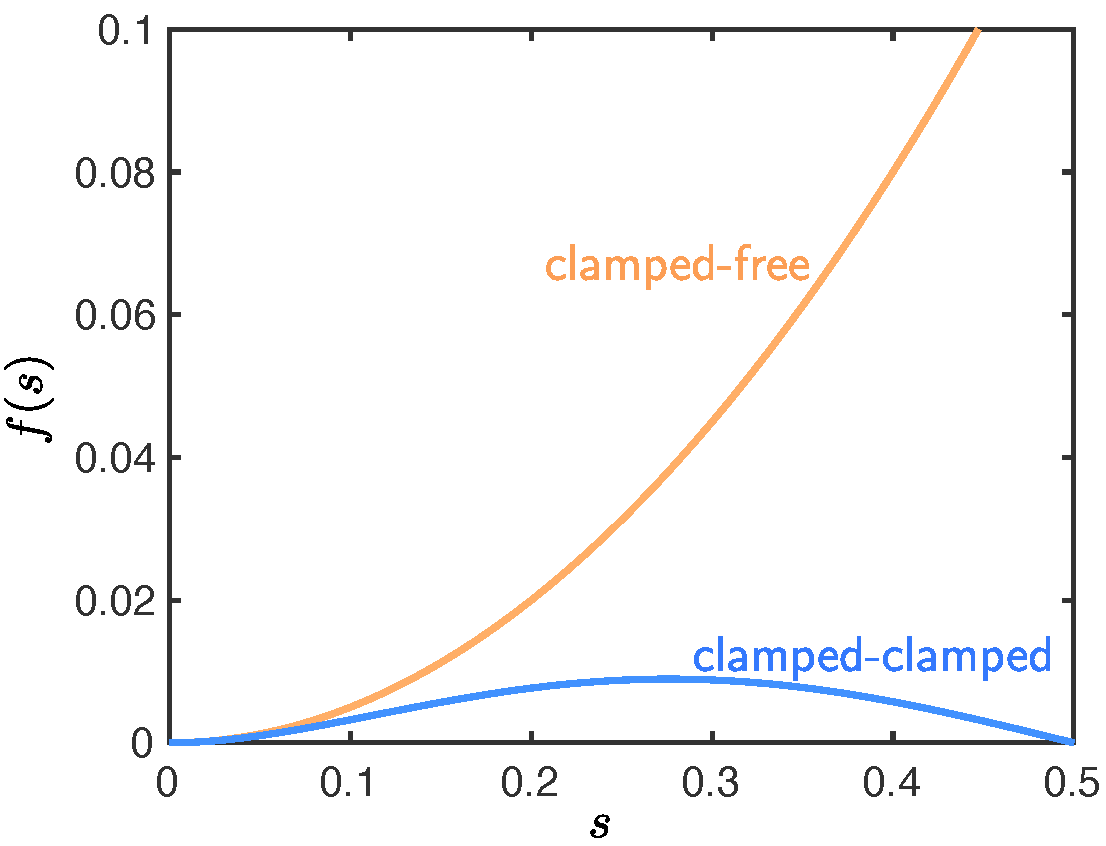
\includegraphics[scale=0.4]{doubly_clamped}
\caption{Plot of the functions $f = f_{\text{clamped}}$ and $f = f_{\text{free}}$ (defined in~\eqref{A:E:Ch2:SmallDroplets:DoublyClamped:xm_ODE_functions}) which describe the speed of small droplets in deformable channels in which both ends are clamped (blue curve) and in channels in which one end is clamped and the other is free (orange curve).}\label{fig:Ch2:Appendix:doubly_clamped}
\end{figure}

In our experimental study of bendotaxis in the following chapter, we encounter the problem of a droplet in a channel that is clamped at both ends. In this section, we consider the behaviour of such a configuration in the case that the droplet is small, $V\ll 1$.

The problem is the same as that in the previous sections of this appendix, but with the free end conditions at $x = 1$ replaced by clamped conditions:
\begin{equation}
h = 0 = \ddp{h}{x} \qquad \text{at}~x = 1.
\end{equation}

We proceed in the same manner as in the clamped-free case of A.1--A.2 by deriving a point force problem. The analysis of Appendix \ref{A:Ch2:SmallDroplets:SmallVolumeExpansion} (in particular, the ODE~\eqref{A:E:Ch2:SmallDroplets:ReducedKinematic}) is still applicable. As we shall see, the jump conditions~\eqref{A:E:Ch2:SmallDroplets:Slope_and_moment_small} are still applicable, but because of the different boundary conditions at $x = 1$, they require a different justification.  Note, however, that to justify the jump conditions on the first and second derivatives (equation~\eqref{A:E:Ch2:SmallDroplets:PtForceJump}) it is sufficient to show that the moment and shear are $\mathcal{O}(V)$.

To make this justification, we first note that the clamped end at $x = 1$ results in effective boundary conditions
\abeqn{A:E:Ch2:SmallDroplets:DoubleClamped:EffBCXright}{
\ddp{^2 h}{x^2} = \frac{2}{\xright^2}\left(2\xright \ddp{h}{x} - 3h + 3\right), \quad \ddp{^3 h}{x^2} = \frac{6}{\xright^3}\left(\xright \ddp{h}{x} - 2h + 2\right)}
at $x = \xright$ (as discussed in \S\ref{S:Ch2:Numerics:Scheme} for the clamped end at $x = 0$).

Let us assume that the channel slope remains small  $\partial h_1 /\partial x = \mathcal{O}(1)$; as we shall see, this is satisfied provided that $\nu = \mathcal{O}(1)$.  Inserting the small deflection ansatz~\eqref{A:E:Ch2:SmallDroplets:Expansion} into~\eqref{A:E:Ch2:SmallDroplets:DoubleClamped:EffBCXright} gives
\begin{equation}
\left.\ddp{^2 h}{x^2}\right|_{x = \xright} =\left. \frac{2}{\xright^2}\left[2\xright V\ddp{h_1}{x} - 3(1 + V h_1) + 3\right]\right|_{x = \xright} + \mathcal{O}(V^2)  =   \mathcal{O}(V)
\end{equation}
and
\begin{equation}
\left.\ddp{^3 h}{x^3}\right|_{x = \xright} =\left. \frac{6}{\xright^2}\left[\xright V\ddp{h_1}{x} - 2(1 + V h_1) + 2\right]\right|_{x = \xright} + \mathcal{O}(V^2)  =   \mathcal{O}(V).
\end{equation}
The moment and shear at $x  = \xright$ are both therefore $\mathcal{O}(V)$ as required, and so the jump conditions across the droplet are identical for both the clamped-clamped and clamped-free configurations.

The leading order point force problem for $h_1$ in the clamped-clamped configuration is therefore
\begin{equation}\label{A:E:Ch2:SmallDroplets:DoublyClamped:PtForcePDE}
\ddp{^4 h_1}{x^4} = 0, \qquad \text{in}~0< x < \xright,~\text{and}~\xright < x < 1,
\end{equation}
with jump conditions
\begin{equation}\label{A:E:Ch2:SmallDroplets:DoublyClamped:PtForceJump}
\left[\ddp{^3 h_1}{x^3}\right]_{\xright^-}^{\xright^+} = -\nu, \qquad \left[\ddp{^2 h_1}{x^2}\right]_{\xright^-}^{\xright^+} =0, \qquad \left[\ddp{ h_1}{x}\right]_{\xright^-}^{\xright^+} =0,\qquad \left[h_1\right]_{\xright^-}^{\xright^+} = 0,
\end{equation}
and boundary conditions
\begin{equation}\label{A:E:Ch2:SmallDroplets:DoublyClamped:PtForceBC}
h_1 = 0 = \ddp{h_1}{x}, \qquad\text{at}~x = 0, 1.
\end{equation}

The solution to~\eqref{A:E:Ch2:SmallDroplets:DoublyClamped:PtForcePDE}--\eqref{A:E:Ch2:SmallDroplets:DoublyClamped:PtForceBC} is
\begin{equation}\label{A:E:Ch2:SmallDroplets:DoublyClamped:SolutionShape}
h_1(x,t) = \begin{cases}{}
       1 + Ax^2 + Bx^3& \text{for }\quad 0 < x < \xright(t), \\
  1 + C(1-x)^2 + D(1-x)^3& \text{for }\quad \xright(t) < x < 1.
        \end{cases}
\end{equation}
where
\begin{align}
A &= -\frac{\nu\xright}{2} \left(\xright^2 + 2\xright -1\right),&  B &= \frac{\nu}{6}\left(2\xright^3 - 3\xright^2 + 1\right),\label{A:E:Ch2:SmallDroplets:DoublyClamped:SolutionShapeCoeffs1}\\
C &= \frac{\nu\xright^2}{2}\left(\xright -1\right), & D&= -\frac{\nu\xright^2}{2}\left(\xright -1\right)\label{A:E:Ch2:SmallDroplets:DoublyClamped:SolutionShapeCoeffs2}
\end{align}
(The solution~\eqref{A:E:Ch2:SmallDroplets:DoublyClamped:SolutionShape} informs us that the channel slope remains small, $\partial h/\partial x \sim \mathcal{O}(V)$, provided that $\nu =  \mathcal{O}(1)$).

Inserting~\eqref{A:E:Ch2:SmallDroplets:DoublyClamped:SolutionShape}--\eqref{A:E:Ch2:SmallDroplets:DoublyClamped:SolutionShapeCoeffs2} into the kinematic condition~\eqref{A:E:Ch2:SmallDroplets:ReducedKinematic} gives the ODE
\begin{equation}\label{A:E:Ch2:SmallDroplets:DoublyClamped:xm_ODE}
\dd{\xright}{t} = \frac{\nu V}{6}\frac{\xright^2(1-2\xright) (\xright -1)^2}{2}.
\end{equation}
Note that~\eqref{A:E:Ch2:SmallDroplets:DoublyClamped:xm_ODE} is anti-symmetric about $\xright = 1/2$, so the system is in equilibrium when the droplet sits at the centre of the channel. Furthermore, the channel deformation is maximised when the droplet sits at the centre, with deformation
\begin{equation}\label{A:E:Ch2:SmallDroplets:DoublyClamped:first_order_deformation}
1 - h(x = 1/2,t) = \frac{V \nu}{192}.
\end{equation}

Figure~\ref{fig:Ch2:Appendix:doubly_clamped} compares the functions
\begin{equation}\label{A:E:Ch2:SmallDroplets:DoublyClamped:xm_ODE_functions}
f_{\text{clamped}}(s) = \frac{s^2(2s-1)(s-1)^2}{2}, \quad \text{and}\quad f_{\text{free}}(s) = \frac{s^2}{2},
\end{equation}
which describe how the speed of the meniscus changes as the droplet moves along the channel (see equations~\eqref{A:E:Ch2:SmallDroplets:xrightODE} and~\eqref{A:E:Ch2:SmallDroplets:DoublyClamped:xm_ODE}). We note that $f_{\text{free}}(s) > f_{\text{clamped}}(s)$ throughout $|s| < 1/2$, and conclude that motion is always quicker when the end $x = 1$ is free, rather than clamped, in the small $V$ case. In particular, for $\xright > 0.37$, the motion in the clamped-clamped case will be at least an order of magnitude slower than that with a free end.

In addition
\begin{equation}\label{A:E:Ch2:SmallDroplets:DoublyClamped:xm_ODE_function_expansion}
f_{\text{clamped}}(s) \sim \frac{1}{16}\left(s - \frac{1}{2}\right) \qquad \text{as}~s \to \frac{1}{2},
\end{equation}
so the droplet approaches the equilibrium at $\xright = 1/2$ like
\begin{equation}\label{A:E:Ch2:SmallDroplets:DoublyClamped:xm_ODE_function_expansion_result}
\xright -\frac{1}{2}\sim \exp \left(-\frac{\nu V t}{48}\right).
\end{equation}
Returning to dimensional units, equation~\eqref{A:E:Ch2:SmallDroplets:DoublyClamped:xm_ODE_function_expansion_result} means that the time scale of relaxation to equilibrium in the doubly clamped channel is
\begin{equation}\label{A:E:Ch2:SmallDroplets:DoublyClamped:xm_ODE_relaxation_timescale}
T =\frac{48}{\nu V t_c}= \frac{48\mu B H}{\gamma^2 \cos^2 \theta_e \Delta X L}.
\end{equation}
We will return to~\eqref{A:E:Ch2:SmallDroplets:DoublyClamped:first_order_deformation} and~\eqref{A:E:Ch2:SmallDroplets:DoublyClamped:xm_ODE_relaxation_timescale} in the following Chapter.

\end{subappendices}
